\documentclass{my_paper}
\usepackage{ctex}
\usepackage[textwidth=444bp,vmargin=2.5cm]{geometry}%设置页边距
\usepackage{array} %主要是增加列样式选项
\usepackage[dvipsnames]{xcolor}%颜色宏包
\usepackage{graphicx}%图片宏包
\usepackage{amsmath}%公式宏包
\usepackage[T1]{fontenc}    
\usepackage{newtxtext, newtxmath}  %两种使用Times New Roman 字体的方法
\usepackage{subfigure}
\usepackage{tabularx, booktabs} %% Load packages that you use
\usepackage{multirow} %跨行处理
\usepackage{rotating}%横向表格
\usepackage{diagbox}%斜线划分表头

\usepackage { gensymb }
% 打°符号\degree
\usepackage{framed}
\usepackage{listings}
% 代码
\usepackage{color} %red, green, blue, yellow, cyan, magenta, black, white
\usepackage[numbered,framed]{matlab-prettifier}%matlab 代码高亮
\usepackage{mdframed}%另一个边框
% matlab代码样式,使用方法为:
% \lstinputlisting[style=Matlab-editor,linewidth=\textwidth]{code.m}
% 或:
% \begin{lstlisting}[style=matlab-prettifier]
%     %code
% \end{lstlisting}
\renewenvironment{framed}[1][\hsize]
  {\MakeFramed{\hsize#1\advance\hsize-\width \FrameRestore}}%
  {\endMakeFramed}
%   修正framed环境,使之可以变长,用法:
%   \begin{framed}[1.2/textwidth]...

\usepackage{hologo}
\usepackage{gbt7714}
\bibliographystyle{gbt7714-numerical}
% 采用国标参考文献引用
\newcommand{\lunwenbiaoti}{\fontsize{15.75pt}{0}\heiti 基于k-means的古代玻璃分类与成分复原模型}
\newcommand{\zhaiyao}{\fontsize{14pt}{0}\heiti 摘要}
\usepackage{longtable}
\begin{document}

\lstdefinestyle{python_style}{
 columns=fixed,
 numbers=left,                                        % 在左侧显示行号
 numberstyle=\tiny\color{gray},                       % 设定行号格式
 frame=trbl,                                        % 单线背景边框
 breaklines=true,                                     % 设定LaTeX对过长的代码行进行自动换行
 keywordstyle=\color[RGB]{40,40,255},                 % 设定关键字颜色
 numberstyle=\footnotesize\color{darkgray},
 commentstyle=\it\color[RGB]{0,96,96},                % 设置代码注释的格式
 stringstyle=\rmfamily\slshape\color[RGB]{128,0,0},   % 设置字符串格式
 showstringspaces=false,                              % 不显示字符串中的空格
 language=python,                                        % 设置语言
 basicstyle=\linespread{1.0}\fontsize{10bp}{10bp}\selectfont\ttfamily,                      % 字体字号
 %lineskip=10bp,
 %baselinestretch=1,
}
\newpage
\begin{center}
\lunwenbiaoti

\vspace{2ex}
\zhaiyao
\end{center}

丝绸之路上玻璃是重要的运输商品,沿线国家的文化交流的过程中留下了许多玻璃文物,因而对于玻璃文物的成分分析和分类具有重要的考古价值。我们首先利用方差分析得出种类同风化之间的显著关系;为了得到风化前的玻璃成分,使用综合变化比例求取风化前的元素比例;使用投票法建立大类划分模型,以及k-means方法建立亚类的划分模型;最后探究了成分之间单变量与多变量的相关关系,并使用R-square来衡量拟合结果。

针对问题一,我们首先对数据进行数据清洗和确实填补可视化分析,统计均值、方差与变异系数等指标,分析数据的分布情况;其次,我们探究纹饰、颜色和类型三指标与风化间的关系,使用方差分析法得出类型与风化之间的相关程度最高,并使用卡方分布验证了该结果。

为了预测风化前的成分含量,利用数据的不同样本,综合样本间变化比例与跨样本的变化比例,计算原有成分。为了验证结果的好坏,将预测未风化数据与原始未风化数据作为标签,利用皮尔逊相关系数分析标签与数据之间的相关性,验证出预测结果有效。

针对问题二,我们统计未风化前玻璃样本各个化学指标的含量分界,使用分界上的倾向加权投票,得出最终分类结果。经过验证,大类划分过程达到了$98.44\%$的准确度。

在亚类划分的过程中,使用变异系数与相关的文献资料确定分类的参考指标。使用k-means++方法进行聚类,并使用F相关系数同样本含量的显著性水平作为评价k值好坏的标准,最终确定了铅钡玻璃划分6类,高钾玻璃划分5类作为最优的类别划分数目。在得到划分结果后,对亚类划分的合理性做出解释,并利用原始数据波动的方式测试了亚类分类的敏感性,亚类均表现出较高的稳定性。

针对问题三,我们首先对风化数据进行还原,并利用问题二中的划分模型做大类和亚类的分析,并且测试在分界数据和类中心发生变化时,分类结果的稳定性。

针对问题四,首先使用皮尔逊相关系数和最大信息系数来评价各成分两两之间的相关程度。再挑出相关程度较大的成分组合。我们使用各种常见的函数拟合两变量之间的关系,并用R-square来衡量拟合效果,最后选用优度最高的拟合函数作为成分之间的定量关系。对于多指标的关系确定,我们选取相互相关性均较强的几组成分,采用多元线性拟合方式对其拟合,最终确定其关系。

本文采用多种相关检验方法,对假设进行检验,且重要结果均列表或绘图呈现,较为直观。

\begin{guanjianci}
 方差检验 \quad k-means \quad 皮尔逊相关检验
\end{guanjianci}

%----------- 正文 ----------
%----------- 一、问题重述 ----------
\newpage
\section{一、问题重述}

\subsection{问题背景}

我国具有悠久的玻璃制作历史,玻璃是丝绸之路历史的重要物证,在考古工作中,需要对玻璃的成分进行分析,并对其种类进行鉴别。

玻璃以石英砂(主要成分为$SiO_2$)作为主要原料,在制造的过程中为了降低熔点,添加不同的助熔剂进行炼制,并加入氧化钙等作为稳定剂。根据所加入助熔剂的不同,玻璃化学成分产生差异,这使得古代玻璃产生了不同的种类。例如添加铅矿石作为助熔剂的玻璃含有较高的氧化钡和氧化铅含量,常被称作铅钡玻璃;添加草木灰等作为助熔剂的玻璃,具有较高的钾含量,被称作是钾玻璃。

古代玻璃经由漫长的埋藏过程而导致风化。风化的本质是玻璃与外界环境之间产生了元素交换,导致成分发生变化。风化过程的程度不同,导致玻璃的成分,颜色发生较大变化,给考古工作带来了一定困难。
我们需要利用古代玻璃采样的化学检测数据,探究风化与物质成分的变化关系,以及分类标准与成分之间的相关关系。

\subsection{问题重述}
经过分析整理,我们需要解决以下问题:
\begin{enumerate}
    \item 分析表面风化同玻璃类型、纹饰和颜色之间的关系进行分析,并就类别分析其风化前后的化学含量统计规律,最后根据风化点的检测数据预测未风化前的物质含量。
    \item 分析高钾玻璃和铅钡玻璃之间的类别划分规律,对每个类别选择合适的指标进行亚类的划分,给出划分的结果,并对结果进行敏感性分析。
    \item 对所给附件中未知类别的玻璃文物化学成分进行分析,鉴定所属类别,并对分类结果进行敏感性分析。
    \item 针对不同类别的玻璃文物样品,在不同的化学成分中分析关联关系,对这一关系的差异程度进行分析。
\end{enumerate}
\section{二、问题分析}
\subsection{问题一的分析}

为了解决第一小问,我们首先对原始数据进行清洗,对不满足成分性要求的数据进行剔除。为了分析便面风化与类型、纹饰、颜色之间的关系,考虑使用方差分析和卡方检验,分析三个因素与风化之间的关系。

对于统计规律,我们按照两个不同的类别,除了选取较常见的统计量外,还选择了变异系数来反应含量相差较大的成分的统一波动情况、选取最大最小值反应两类各成分的范围,同时分析了每个成分风化前后的均值变化情况。

为了预测部分玻璃风化前的成分含量,我们先得出两类玻璃风化前相对于风化后的均值变化程度,同时利用原始数据中高钾玻璃的对照组,即同一个玻璃上的风化前和风化后的部位,找到第二个改变程度参考值。最后我们将两个改变量通过赋权的方式结合在一起,预测高钾玻璃风化前成分组成,铅钡玻璃没有对照组,所以只使用第一个变化程度预测。

\subsection{问题二的分析}

为了探寻两类玻璃的分类规律,我们先将风化后的数据还原为风化前的数据,然后计算各个成分在两类玻璃中的相对差值,并依据相对差值为各个成分打出分数,作为此成分区分两类玻璃的重要程度。再计算出两类玻璃各成分的分界线,对于两类玻璃之间含量没有重合的成分,我们采用两类中最邻近的两个样本此成分含量的均值为分界线,对于两类玻璃含量有所重合的成分,我们采用两类玻璃此成分含量的类均值的均值作为分界线。

为了在每个大类下继续划分出亚类,我们挑选出对划分亚类有重要影响的指标,再用kmeans++进行聚类,利用卡方分布的相关性系数检验聚类的合理性,最终采用合理性最强的聚类结果作为最终结果,并依据文献中亚类的名命方式选取每一类中含量较大的一或两个指标来对亚类进行命名。最后,通过上下浮动原始数据重新进行分类方法来分析模型灵敏度。

\subsection{问题三的分析}
利用问题二中找出的大类分类规律,将待分类玻璃的各成分依据其靠近分界线哪一边来赋给此待分类玻璃不同的初始值,并利用问题二中算出的各分界线的相对分数乘以此值,最后将所有成分的得分加和,最终得分更靠近哪个类的成分初始值,此待测玻璃就属于那一大类。因为分界线是从统计数据中得到的,所以具有一定的不确定性,我们通过上下浮动各个分界线重复分类方法来分析模型敏感性。
\subsection{问题四的分析}
为了探寻各类玻璃文物样品中不同化学成分的关联关系,我们将所有样品按高钾玻璃和铅钡玻璃、未风化和风化后,为标准分成四类。首先使用皮尔逊相关系数和最大信息系数来评价各成分两两之间的相关程度。再挑出相关程度较大的成分组合。关于两个指标的关系确定,我们使用各种常见的拟合函数进行拟合,最后用R-square来衡量拟合效果,并选用优度最高的拟合函数作为成分之间的定量关系。对于多指标的关系确定,我们选取相互相关性均较强的几组成分,采用多元线性拟合方式对其拟合,最终确定其关系。
%----------- 三、模型假设 ----------
\section{三、模型假设}
%使用代码片段:、jiashe%
\begin{enumerate}
    \item 假设各个样本是独立同分布的
    
 


\end{enumerate}

%----------- 四、符号说明 ----------
\section{四、符号说明}
%使用三线表格最好~


以下是本文使用的符号以及含义:
\begin{table}[h]%htbp表示的意思是latex会尽量满足排在前面的浮动格式,就是h-t-b-p这个顺序,让排版的效果尽量好。
    \centering
    \begin{tabular}{p{2.0cm}<{\centering}p{9.0cm}<{\centering}p{2.0cm}<{\centering}}
 %指定单元格宽度, 并且水平居中。
    \hline
    符号 & 说明 & 单位 \\ %换行 
    \hline
    $c$ & 化学元素含量 &  $\%$\\
    $\Delta$ & 化学元素变化量 &  $\%$\\
    $c_v$ & 变异系数 &  /\\
    $B$ & 铅钡玻璃下标 & / \\
    $K$ & 高钾玻璃下标 &  \\
    \hline
    \end{tabular}
\end{table}

%----------- 五、模型的建立与求解 ----------
\section{五、模型的建立与求解}

以下将对提出的四个问题进行建模求解。
\subsection{数据清洗与可视化分析}
在这一部分,我们进行了一些数据预处理工作。首先对剔除不满足要求的数据,随后对缺失的数据进行填补,最后将数据进行分析统计,以更好的进行建模活动。

\subsubsection{剔除异常数据}
根据题目信息,需要对不满足成分性的数据进行剔除。成分性的定义为各个成分之间的加和应该是等于$ 100\% $,但是由于种种因素这一性质不能达到。规定各个组分的加和处于$85\%\sim 105\%$之间的数据作为有效数据。对表单2中的69条数据进行统计,得到图(\ref{51})所示的结果。
\begin {figure}[h]
\centering % 居中显示
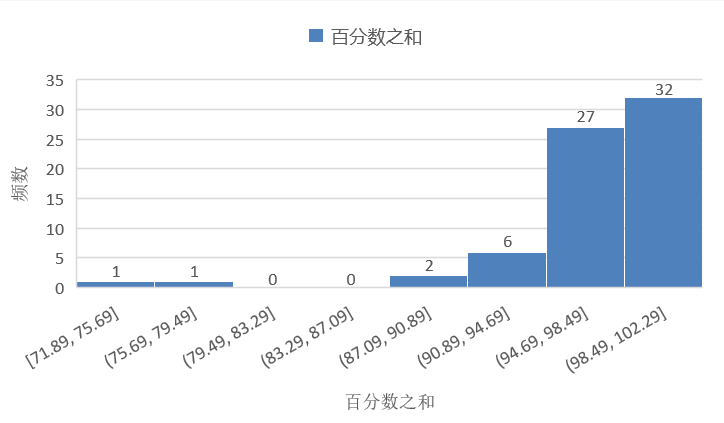
\includegraphics[width=0.7\textwidth]{51.png}
\caption{附件二各采样点成分的求和} % 标题
\label{51}
\end {figure}

可见数据总体分布在$87.09\%\sim 102.29\%$这一区间中,只有两条记录不能满足成分性,分别是17号采样点$71.89\%$以及15号采样点$79.47\%$,将其剔除。

\subsubsection{数据填补}
在58份样本数据中分别说明了其编号、纹饰、类型、颜色与风化程度五项数据,其中颜色一项有四条缺失,分别位于编号 19 、40、 48和58处。为了便于后续的分析处理,将缺失项用“未知”填补,补全了数据缺口。

\subsubsection{可视化分析}
为了便于后续的分析处理,我们对数据进行可视化分析。为了判断类别分布的规律,首先对文物样本在各个指标的分布情况进行分析,得到图(\ref{513})所示的结果。
\begin{figure}[htbp]
    \centering  %居中
    \subfigure[纹饰分布]{   %第一张子图
    \begin{minipage}{0.35\textwidth}%大小总和超过textwidth则自动换行
    \centering    %子图居中
    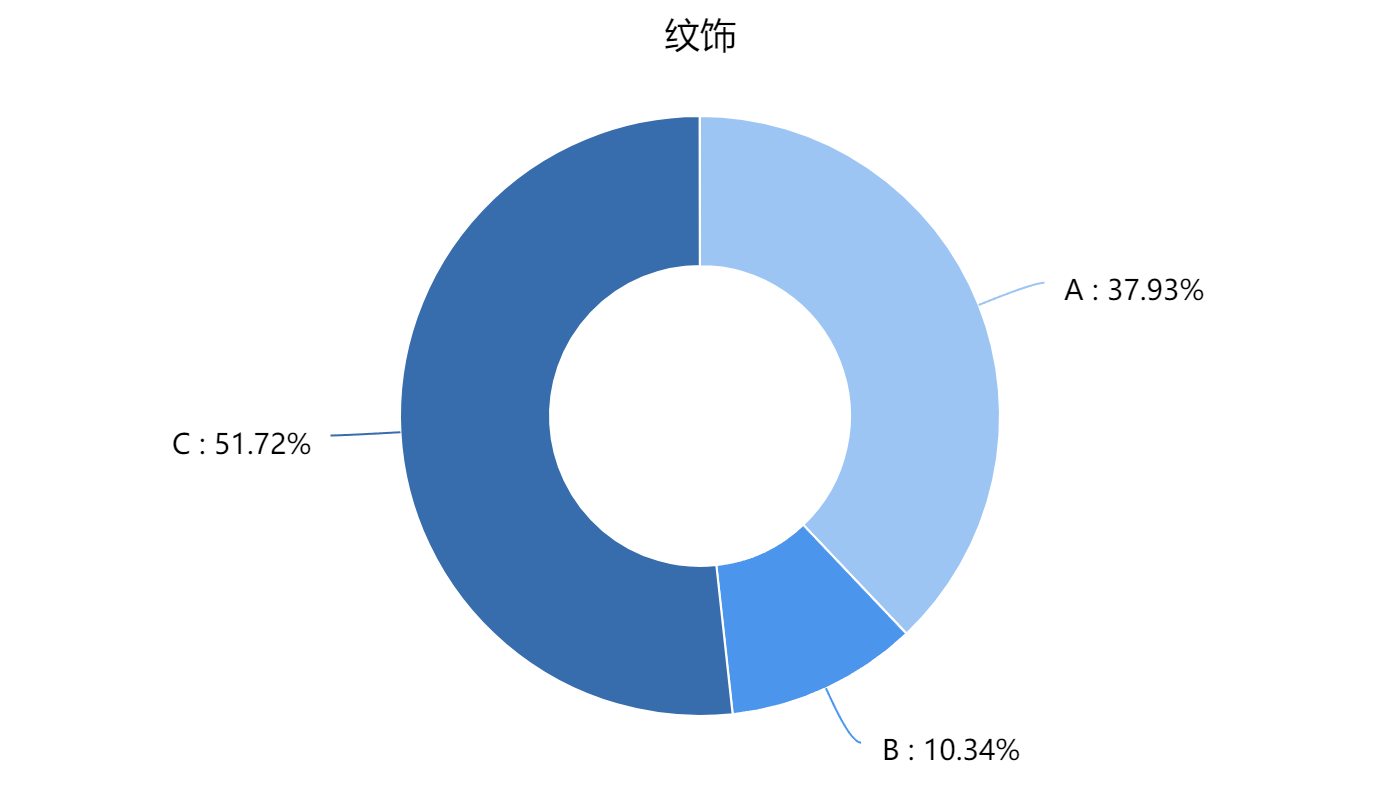
\includegraphics[width=\textwidth]{513ws.png}  %设置图片的输出大小倍数,这里是0.5倍大小输出
    \end{minipage}
    }
    \subfigure[类型分布]{   %子图
    \begin{minipage}{0.35\textwidth}%大小总和超过textwidth则自动换行
    \centering    %子图居中
    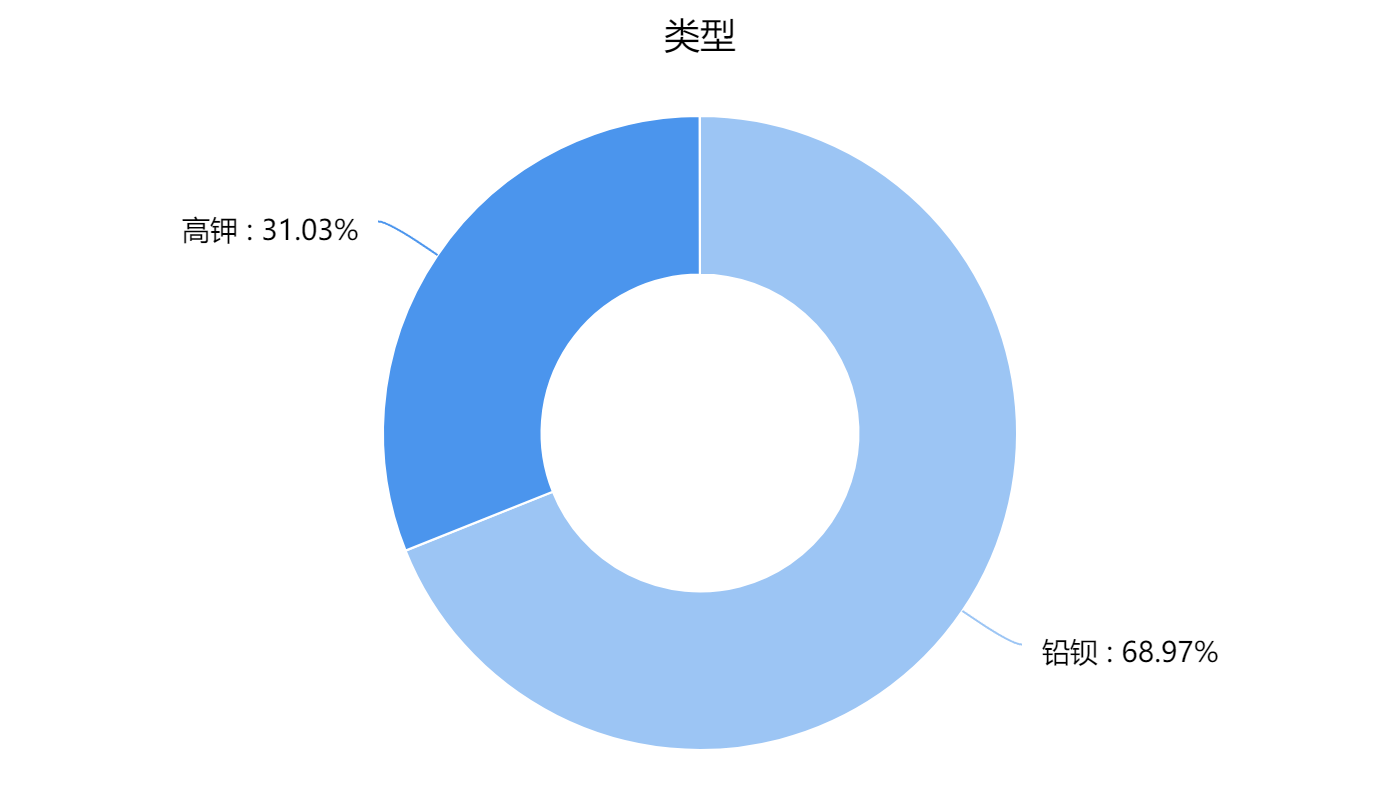
\includegraphics[width=\textwidth]{513lx.png}  %设置图片的输出大小倍数,这里是0.5倍大小输出
    \end{minipage}
    }\\
    \subfigure[颜色分布]{ %第二张子图
    \begin{minipage}{0.5\textwidth}
    \centering    %子图居中
    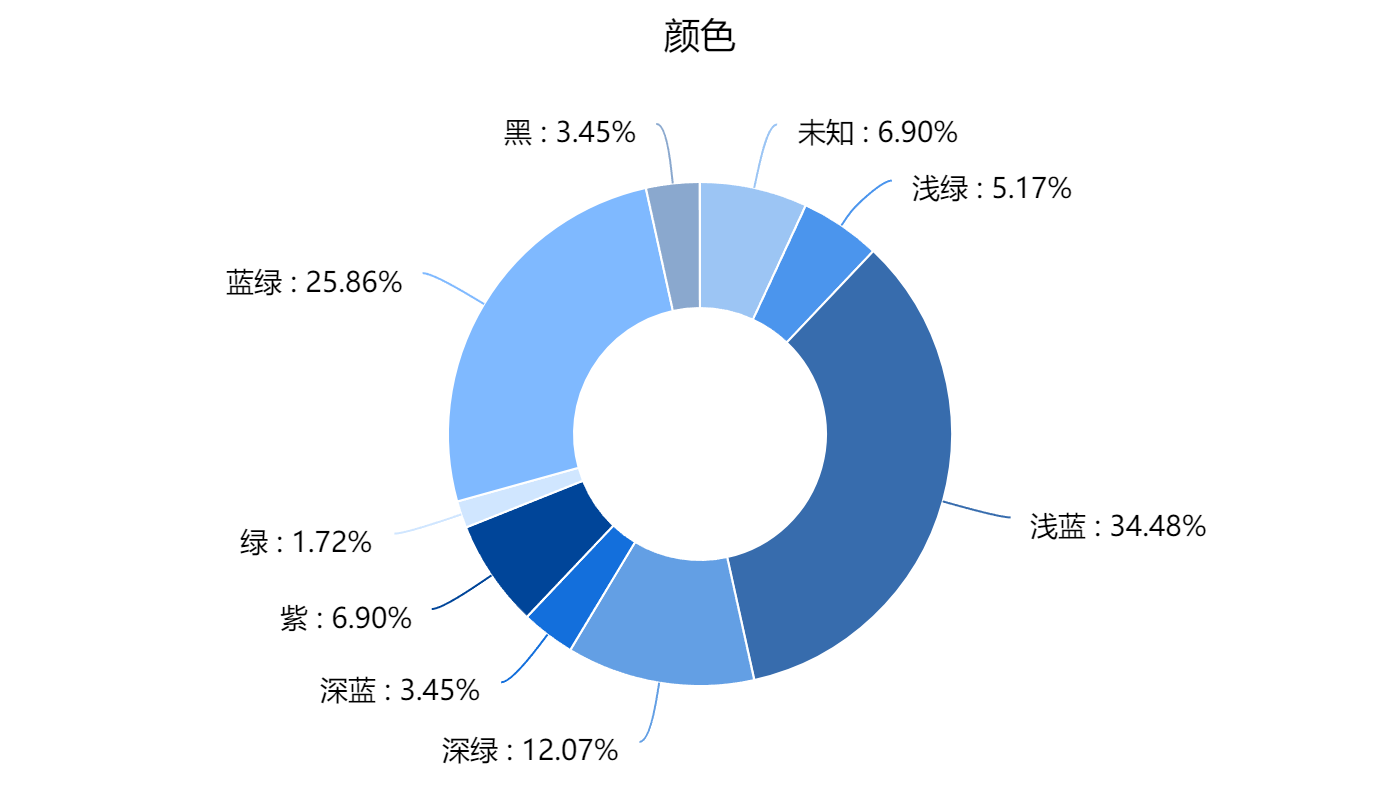
\includegraphics[width=\textwidth]{513ys.png}%以pic.jpg的0.5倍大小输出
    \end{minipage}
    }
    \caption{玻璃样本基本信息的分布情况}    %大图名称
    \label{513}    %图片引用标记
\end{figure}
可见古代玻璃样本以C类型的纹饰为主,其次是A纹饰,B纹饰的占比最小,仅占$10.34\%$。在类型分布上,铅钡玻璃的占比超过了三分之二,成为数量较多的一类。在颜色分布上,颜色以蓝、绿为主,可能是由于其中的$Fe^{3+}$,$ Cu^{2+} $等离子的存在而显色\cite{3}。其中颜色由显现出不同的深浅,可能代表显色物质的组合以及浓度差异。
\subsection{古代玻璃风化预测模型}
在本部分,我们首先对古代玻璃的种类、纹饰和颜色,同风化的相关关系进行分析,利用多种方法分析出与风化关系密切的因素。随后我们就玻璃种类和风化与否来划分成分含量指标,给出成分的统计规律,随后建立模型,对古代玻璃的未风化前的元素含量做出预测。

\subsubsection{古代玻璃各指标同风化间相关性分析}
为了探究古代玻璃的纹饰种类、类型与颜色等因素的差异对于玻璃风化程度的影响,对这三个因素进行相关性分析。我们首先使用方差分析\cite{2}检验相关性。下面以检验纹饰同风化之间的关系叙述计算过程。

我们若将纹饰视作考察的因素,那么不同的纹饰$\{A,B,C\}$则可以视为$r$个不同的水平,这里$r=3$,若用附件所给58个玻璃样本数据进行分析,在各个样本独立同分布的条件下,记录第$k$种纹饰中第$i$个样本的风化程度为$X_{ik}$,每种纹饰的样本数量为$n_A,n_B,n_C$。根据上述信息,可以得到水平项离差平方和(SSA)、误差项离差平方和(SSE)的统计量$SS_A$与$SS_E$:
\begin{equation}
    \mathrm{SS}_{\mathrm{A}}=\sum_{i=1}^{r} \sum_{j=1}^{n_{i}}\left(\bar{X_{i}}-\bar{X}\right)^{2}=\sum_{i=1}^{r} n_{i}\left(\bar{X_{i}}-\bar{X}\right)^{2} 
\label{ssa}
\end{equation}
\begin{equation}
    \mathrm{SS}_{\mathrm{E}}=\sum_{i=1}^{r} \sum_{j=1}^{n_{i}}\left(X_{i j}-\bar{X_{i}}\right)^{2}
    \label{sse}
\end{equation}


方差分析的基本思想是通过水平项离差平方和(SSA)、误差项离差平方和(SSE)的统计量判断假设$H_0$:$\mu_1=\mu_2=\cdots=\mu_r$是否成立。这里的$\mu$代表风化程度的均值。当上述假设成立时满足下式:

$$\frac{\mathrm{SS}_{\mathrm{A}}}{\sigma^{2}} \sim \chi^{2}(r-1), \quad \frac{\mathrm{SS}_{\mathrm{E}}}{\sigma^{2}} \sim \chi^{2}(n-r)$$

样本的方差是未知的变量,构造检验量$F$进行处理,将其消去,得到下式:
\begin{equation}
    F=\frac{\mathrm{SS}_{\mathrm{A}} / \mathrm{df}_{\mathrm{A}}}{\mathrm{SS}_{\mathrm{E}} / \mathrm{df}_{\mathrm{E}}}=\frac{\mathrm{MS}_{\mathrm{A}}}{\mathrm{MS}_{\mathrm{E}}} \sim F(r-1, n-r)
\label{F}
\end{equation}

其中$MS_A$与$MS_E$称作是均方和,以$F$的显著性大小来检验纹饰种类同风化情况之间的关联程度。在给定的显著性水平$\alpha$下,原假设$H_0$的拒绝域为$F\ge F_\alpha(r-1,n-r)$。而对于颜色和类型的水平与风化程度的分析方面,我们可以使用相似的方法进行分析。下面将给出三个指标相关性分析的结果。
经过计算,三个因素的重要参数罗列在表(\ref{fc})中。
% \newpage
\begin{table}[ht]
\centering
\caption{根据类型 、纹饰和颜色的方差分析结果}
\begin{tabular}{c|ccc}
\toprule
\diagbox{指标}{因素}& 类型     & 纹饰      & 颜色     \\\midrule
$SS_A$ & 1.669  & 1.2023  & 2.288  \\
$SS_E$ & 12.4   & 12.8667 & 11.781 \\
$MS_A$ & 1.669  & 0.6011  & 0.2542 \\
$MS_E$ & 0.2214 & 0.2339  & 0.2454 \\
$F$    & 7.5373 & 2.5697  & 1.0358 \\
\bottomrule
  \end{tabular}
\label{fc}
  \end{table}

  对三个因素在显著性水平$\alpha = 0.01,0.05,0.1$的条件下,查表\cite{4}可知,类型 、纹饰和颜色三个因素所得$F$值在如下对应范围内。注意到由于部分$F_\alpha$的数值没有直接查到,我们利用$F_\alpha$的单调性,使用临近的值进行判断。
  \begin{align}
    F_{\text{类型}}&=7.5373> F_{0.01}(1,40)=7.314 >F_{0.01}(1,57)\\
    F_{\text{纹饰}}&=2.5697< F_{0.05}(2,60)=3.150 <F_{0.05}(2,55)\\
    F_{\text{颜色}}&=1.0358< F_{0.1}(8,60)=1.7745 <F_{0.01}(8,49)
  \end{align}
  分析其结果,可知类型这一因素的差异极显著($\alpha = 0.01$),而其余两个因素的差异性不强,特别是颜色这一因素,没有显著影响。因此我们认为玻璃的种类是影响风化的重要因素,纹饰种类对风化有影响,但是程度不高,颜色与风化之间的关系没有显著关系。

  为了验证所得结果的正确性,使用卡方分布来验证三个因素同风化之间是否呈现出显著性。借助求解器\cite{5},统计了三因素同表面风化的交叉图(图\ref{cro}),此外还计算出$\chi^2$和差异性指标$p$的结果,如表(\ref{chi})所示。
  \begin{figure}[htbp]
      \centering  %居中
      \subfigure[类型]{   %第一张子图
      \begin{minipage}{0.4\textwidth}%大小总和超过textwidth则自动换行
      \centering    %子图居中
      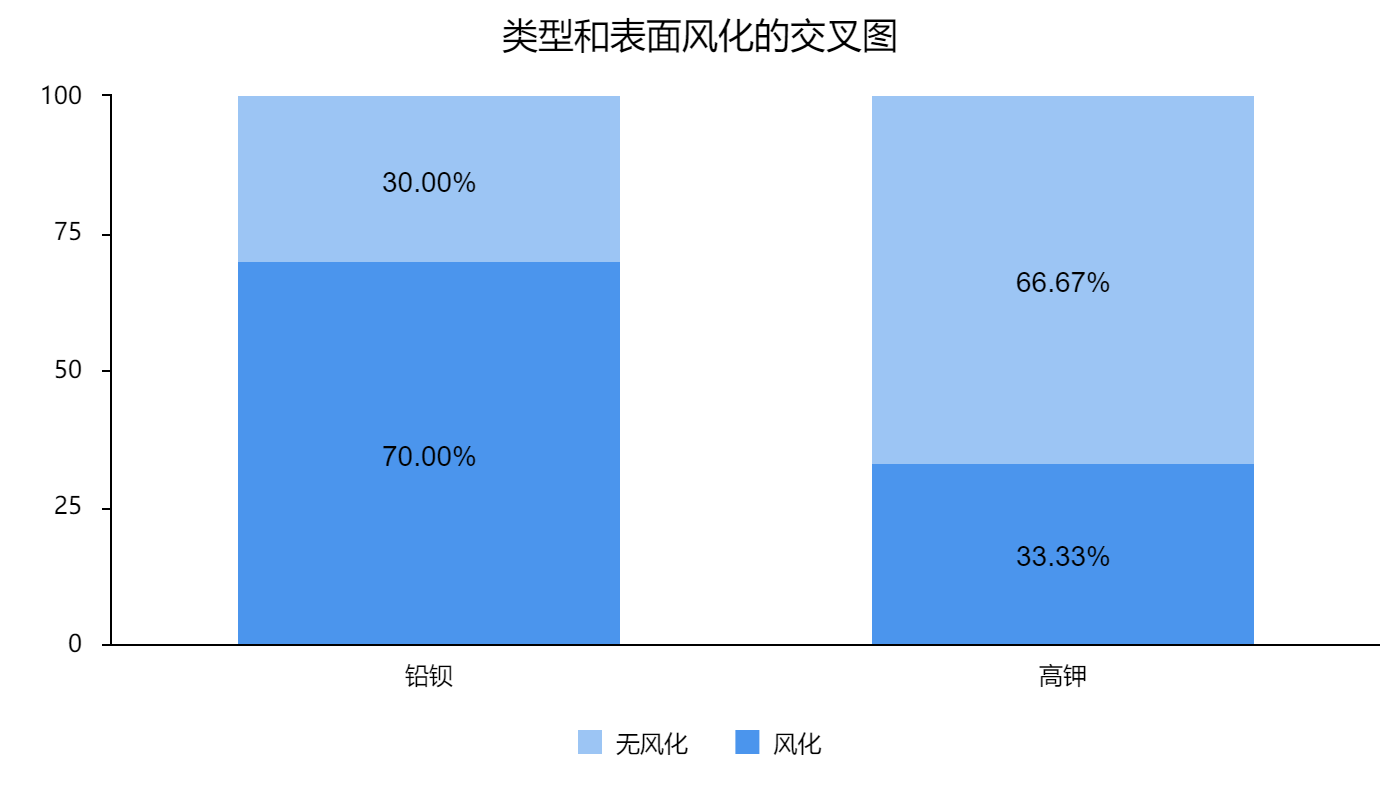
\includegraphics[width=\textwidth]{crolx.png}  %设置图片的输出大小倍数,这里是0.5倍大小输出
      \end{minipage}
      }
      \subfigure[纹饰]{ %第二张子图
      \begin{minipage}{0.4\textwidth}
      \centering    %子图居中
      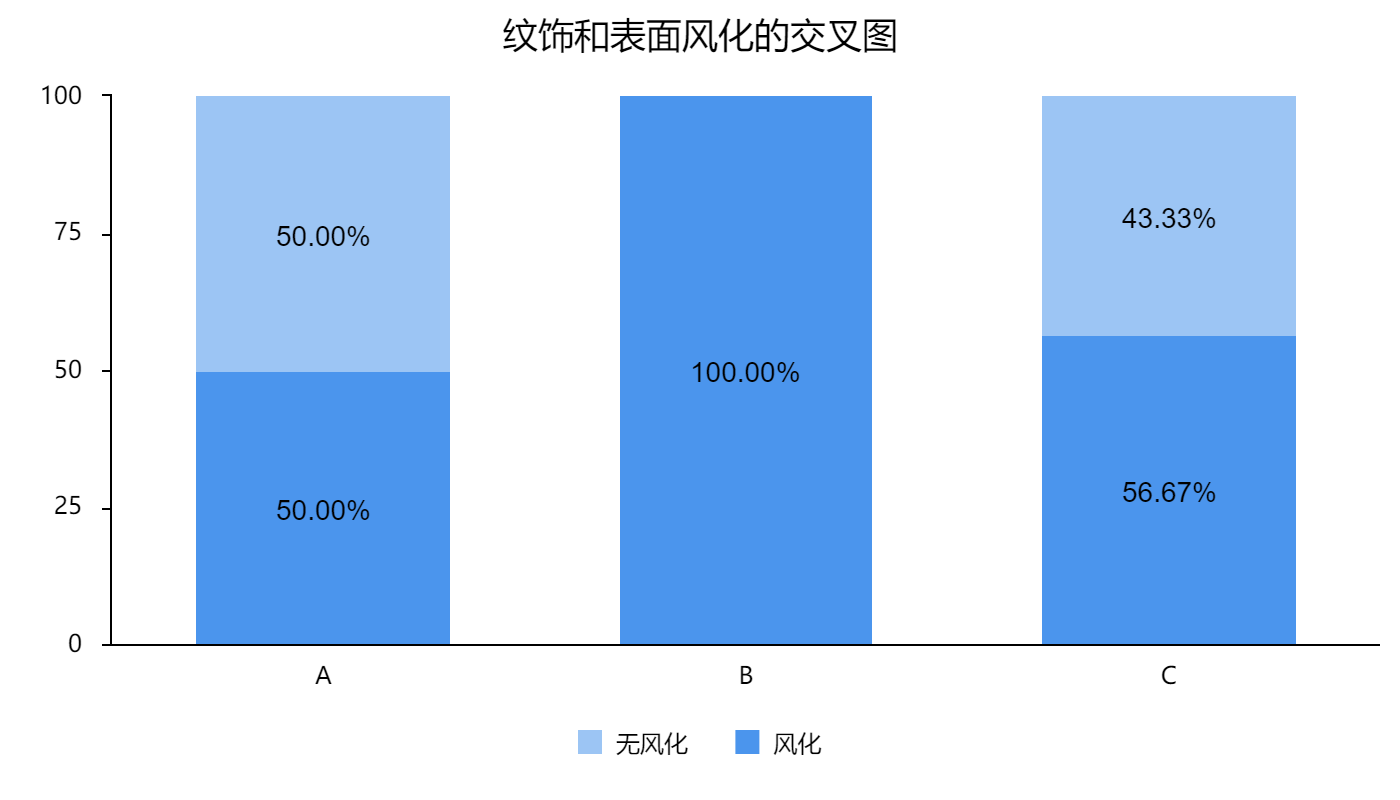
\includegraphics[width=\textwidth]{crows.png}%以pic.jpg的0.5倍大小输出
      \end{minipage}
      }\\
      \subfigure[颜色]{ %第二张子图
      \begin{minipage}{0.4\textwidth}
      \centering    %子图居中
      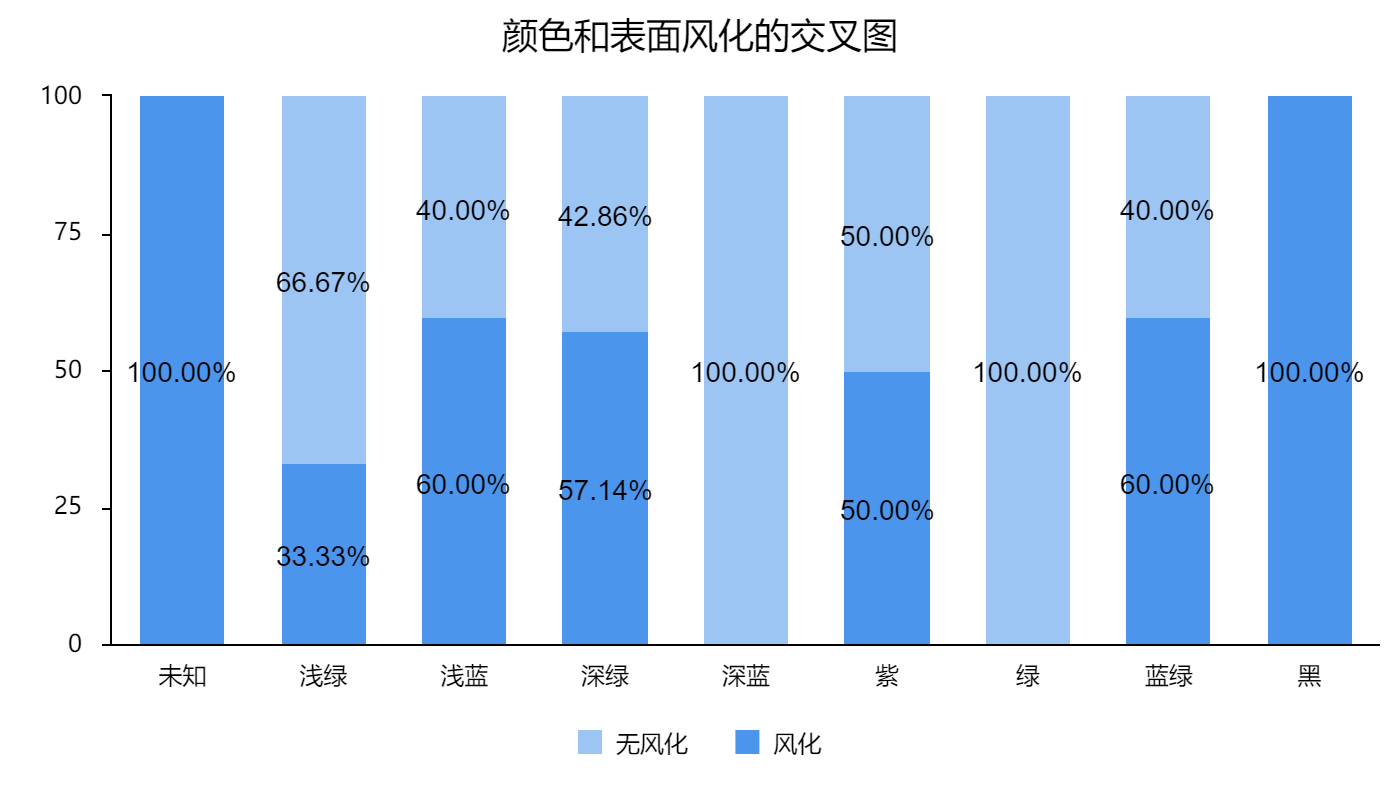
\includegraphics[width=\textwidth]{croys.png}%以pic.jpg的0.5倍大小输出
      \end{minipage}
      }
      
  
      \caption{三个因素同风化程度的交叉图}    %大图名称
      \label{cro}    %图片引用标记
  \end{figure}

  \begin{table}[ht]
  \centering
  \caption{三个因素的卡方分析结果表}
  \begin{tabular}{cccc}
  \toprule
  表面风化因素&$ \chi^2 $&$ p $&显著性\\\midrule
  类型&$ 6.880 $&$ 0.009^{**} $&高显著性\\
  纹饰&$ 4.957 $&$ 0.084 $&无显著性\\
  颜色&$ 9.432 $&$ 0.307 $&无显著性\\
  \bottomrule
    \end{tabular}

    \vspace{2pt}
    注:$*$代表$p<0.05$,说明具有显著性,$**$代表$p<0.01$说明具有高显著性。
  \label{chi}
    \end{table}
    分析结果,可以观察到在三个因素中只有类型产生了高显著性,而纹饰颜色两个因素并未得出显著性结论,分析图(\ref{cro}a)也可直观看出玻璃类型对于风化的结果有明显差异,故可以认为我们所使用的方法具有合理性。

    \subsection{古代玻璃样品统计规律分析}
    考虑到风化过程产生了元素的交换,玻璃风化与否影响着成分含量;与此同时,玻璃的种类也会造成所含物质的差异性。为此,我们将附件表单二中的69条数据按类型和风化程度两个因素,划分为5组:高钾玻璃未风化、高钾玻璃风化、铅钡玻璃未风化、铅钡玻璃风化和铅钡玻璃严重风化。没有出现高钾玻璃的严重风化这一组别是因为原始数据中不存在,故不予记录。
    
    随后计算各个组别的条目数量,均值与方差,最大值和最小值,还有变异系数\cite{6},得出基本的统计结果。计算均值的目的在于统计元素组成的普遍相似性,同时降低那些由于古代工艺所限导致的含量误差。方差反映的是成分的波动程度,由于各个指标的绝对占比有很大不同,其波动程度的衡量可以用变异系数$c_v$这一指标进行衡量,计算式如下。
    \begin{equation}
    c_v = \frac{\sigma}{\mu}
    \label{cv}
    \end{equation}
    其中$ \sigma $代表标准差,$ \mu $  代表均值。最大值最小值反应的是指标占比的分布范围,对于后续分类预测的工作具有较大作用。

    由于全部表的详细信息所占篇幅太大,仅仅选取未风化的高钾玻璃指标条目(表\ref{index1})在正文中展示,其余几类表将在附录中给出。
    \begin{table}[ht]
    \centering
    \caption{未风化高钾玻璃统计量}
    \begin{tabular}{cccccccc}
    \toprule
    名称                   & 样本量                 & 最小值                  & 最大值                  & 平均值                 & 标准差                 & 中位数                 & 变异系数(CV)            \\
    \midrule
二氧化硅(SiO2)           & 12                   & 59.01                & 87.05                & 67.984               & 8.755                & 65.53                & 12.878\%             \\
氧化钠(Na2O)            & 12                   & 0                    & 3.38                 & 0.695                & 1.287                & 0                    & 185.168\%            \\
氧化钾(K2O)             & 12                   & 0                    & 14.52                & 9.331                & 3.92                 & 9.83                 & 42.014\%             \\
二氧化硫(SO2)            & 12                   & 0                    & 0.47                 & 0.102                & 0.186                & 0                    & 182.472\%            \\
氧化钙(CaO)             & 12                   & 0                    & 8.7                  & 5.332                & 3.092                & 6.095                & 57.993\%             \\
氧化镁(MgO)             & 12                   & 0                    & 1.98                 & 1.079                & 0.676                & 1.165                & 62.654\%             \\
氧化铝(Al2O3)           & 12                   & 3.05                 & 11.15                & 6.62                 & 2.492                & 6.185                & 37.636\%             \\
氧化铁(Fe2O3)           & 12                   & 0                    & 6.04                 & 1.932                & 1.667                & 2.11                 & 86.283\%             \\
氧化铜(CuO)             & 12                   & 0                    & 5.09                 & 2.453                & 1.66                 & 2.345                & 67.686\%             \\
氧化铅(PbO)             & 12                   & 0                    & 1.62                 & 0.412                & 0.589                & 0.155                & 143.074\%            \\
氧化钡(BaO)             & 12                   & 0                    & 2.86                 & 0.598                & 0.982                & 0                    & 164.140\%            \\
五氧化二磷(P2O5)          & 12                   & 0                    & 4.5                  & 1.402                & 1.434                & 1.02                 & 102.243\%            \\
氧化锶(SrO)             & 12                   & 0                    & 0.12                 & 0.042                & 0.048                & 0.02                 & 116.157\%            \\
氧化锡(SnO2)            & 12                   & 0                    & 2.36                 & 0.197                & 0.681                & 0                    & 346.410\%            \\
    \bottomrule
      \end{tabular}
    \label{index1}

    注:表中除变异系数外的数据单位为百分比($\%$)
      \end{table}
分析这些指标,注意到最小值不为$0$的成分有两个,意味着在所有的该类样本的中都有出现该成分。存在四个成分的中位数为0,反映出大量样本未检出该成分。

\newpage
为了更好的判断风化前后的成分变化,对风化前后的两类玻璃的均值进行分析得到图(\ref{bqu})。

\begin{figure}[htbp]
    \centering  %居中
    \subfigure[高钾玻璃]{   %第一张子图
    \begin{minipage}{0.8\textwidth}%大小总和超过textwidth则自动换行
    \centering    %子图居中
    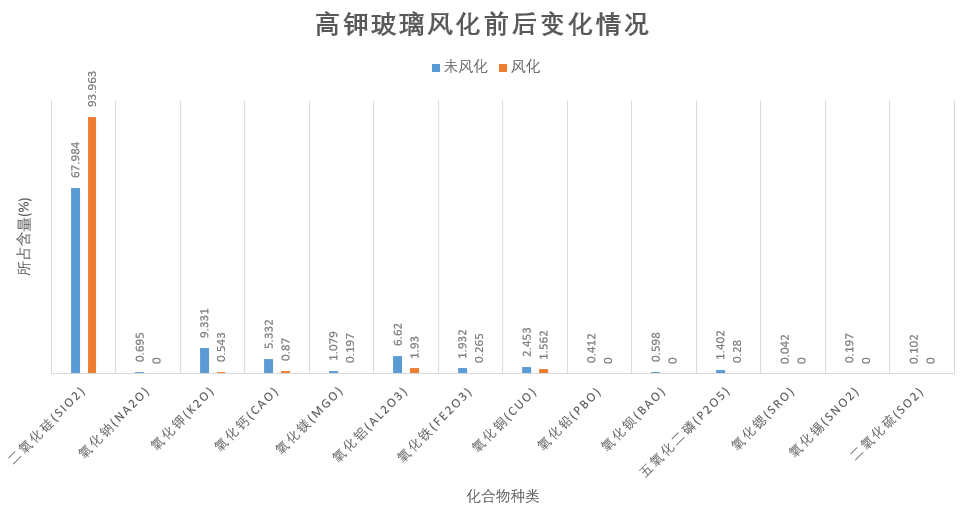
\includegraphics[width=\textwidth]{kqu.png}  %设置图片的输出大小倍数,这里是0.5倍大小输出
    \end{minipage}
    }
    \subfigure[铅钡玻璃]{ %第二张子图
    \begin{minipage}{0.8\textwidth}
    \centering    %子图居中
    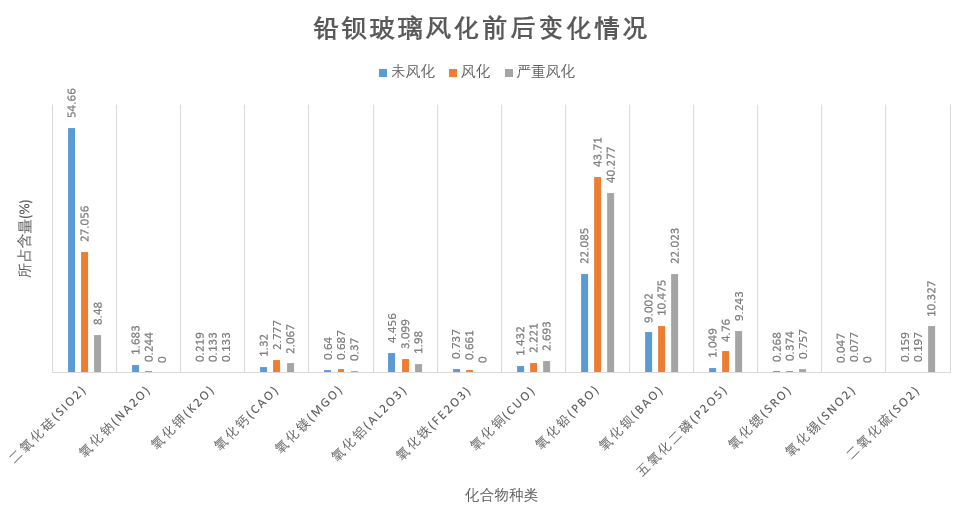
\includegraphics[width=\textwidth]{bqu.png}%以pic.jpg的0.5倍大小输出
    \end{minipage}
    }
    
    \caption{元素变化情况同风化程度的关系}    %大图名称
    \label{bqu}    %图片引用标记
\end{figure}
分析数据,得出玻璃在风化过程中元素占比的变化情况:
\begin{enumerate}
    \item 物质占比在风化过程中随过程的推进,占比呈增加或是减少态势。在风化时玻璃和外界产生物质交换,导致部分物质进入玻璃样品,或是在其余物质流失的情况下,这一物质的占比大大增加。与此同时伴随着随物质流失或是总元素含量增加,部分占比又在随风化程度减少而减少。
    \item 就类间差异而论,高钾玻璃随风化过程的推进,二氧化硅一项的占比在上升,最终达到百分之九十以上,而其余成分都在下降。高钾玻璃的风化过程物质变化较为单一。而铅钡玻璃各项物质的占比变化情况多样,二氧化硅的占比逐步下降,而其余物质如氧化铅,氧化钡,五氧化二磷等在上升。
    \item 由于玻璃所添加的助熔剂不同,在风化前的指标中可以明显看出钾、钡、铅三种氧化物的占比具有很大差异,为后续分类工作提供基础。
\end{enumerate}

\subsection{玻璃样品风化前含量预测模型}
要预测风化样本数据之前的成分占比,在最理想的情况下,需要通过同一样本的风化数据与未风化数据构成一对正反样本。在若干对正反样本中分析风化前后的数据变化,得到稳定结果。鉴于附件数据的特点,风化数据和未风化数据的记录往往位于不同的文物样本,仅有属于铅钡玻璃的49和50号样本满足要求,难以形成成对数据。为此,根据前面分析所得的统计规律,我们提出一种基于均值的原始含量预测模型。

\begin{enumerate}
    \item 跨样本变化比例$\Delta_1$
    
    首先分析不同样本上的风化前后的元素对比,这是因为该部分可利用的数据较多。为了减弱不同古代玻璃样本的成分含量差异,使用均值来计算某一类型的玻璃元素含量多少。若使用$c_{ij}$代表某一类别中第$ i $条记录中的第$ j $项化学成分的占比,那么对于该指标的均值可以使用以下公式计算:
    
    \begin{equation}
    \mu_j = \frac{\sum\limits ^{14}_{j=1}c_{ij}}{n} 
    \label{mu}
    \end{equation}
    ,这里$n$代表采样点记录的数量。如果使用$\mu,\mu'$分别代表风化前与风化后的均值,那么可以计算出跨样本变化比例$\Delta_1$。
    \begin{equation}
    \Delta_1 = \frac{\mu-\mu'}{\mu'}\,,\,\mu'>0
    \label{delta1}
    \end{equation}
    在这里需要处理$ \mu'=0 $的情况,分析数据可知,高钾玻璃的氧化钠(Na2O)
    、氧化铅(PbO)
    、氧化钡(BaO)
    、
    氧化锶(SrO)、
    氧化锡(SnO2)和
    二氧化硫(SO2)五个指标在风化过程中完全流失,无法推知其变化之前的比例。同样地,对于待预测数据中那些流失到0的数据也不能预测其风化前的比例。

    \item 样本内变化比例$ \Delta_2 $
    
    对于同一样本上的不同风化程度数据,同样可以计算其化学成分变化比例,令风化前后的比例分别为$c,c'$,那么可以计算样本内变化比例$ \Delta_2 $:
    \begin{equation}
        \Delta_2 = \frac{\sum\limits_{i=1}^m (c_{ij}-c'_{ij})}{m*c'_{ij}}
    \end{equation}
    其中$ m $为具有正反对比的样本数目,在附件数据中,高钾玻璃$ m=0 $,铅钡玻璃$ m=2 $。

    \item 综合变化比例$ \Delta_0 $
    
    最后我们将综合上述两个指标:跨样本变化比例 $ \Delta_1 $与 样本间变化比例$ \Delta_2 $,将二者以一定比例相加。
    \begin{equation}
        \begin{aligned}
            \Delta_{K0} =& \omega_1 \cdot \Delta_{K1} +\omega_2 \cdot \Delta_{K2} \\            
            \Delta_{B0} =& \Delta_{B1} \\            
        \end{aligned}
    \label{d0}
    \end{equation}
    其中$ \omega $代表权重,$ \Delta_{K}\;,\;\Delta_{B} $分别代表高钾玻璃和铅钡玻璃的变化比例

    在得到综合变化比例$ \Delta_0 $后,给出风化前成分的计算方法。
    \begin{equation}
    c_{ij}^k = \begin{cases}
        (1+\Delta_{K0})*c_{ij}^k&\,,k=K\\
        (1+\Delta_{B0})*c_{ij}^k&\,,k=B\\
    \end{cases} \, \quad , \quad (c_{ij}>0\quad ,\Delta_0 > 0)
    \label{cijk}
    \end{equation}

\end{enumerate}
\subsubsection{模型求解}
经过上述分析和计算,在给定$ \omega_1 = 0.7 $和$ \omega_2=0.3    $的情况下,计算出高钾玻璃和铅钡玻璃各个化学元素的综合变化比例,列出表(\ref{bianhua})。
\begin{table}[ht]
\centering
\caption{各化学成分的变化趋势}
\begin{tabular}{c|ccccc}
\toprule
化学成分                 & \multicolumn{1}{c}{\textbf{二氧化硅(SiO2)}}  & \multicolumn{1}{c}{\textbf{氧化钠(Na2O)}}  & \multicolumn{1}{c}{\textbf{氧化钾(K2O)}}  & \multicolumn{1}{c}{\textbf{氧化钙(CaO)}}  & \multicolumn{1}{c}{\textbf{氧化镁(MgO)}} \\\midrule
$D_{K0}$             &  -0.2765 & Inf      &16.1842 &5.1287 &4.4772\\ 
$D_{B0}$             &  1.0203 &5.8980 &0.6466 &-0.5247 &-0.0684\\\midrule
化学成分                 & \multicolumn{1}{c}{\textbf{氧化铝(Al2O3)}}  & \multicolumn{1}{c}{\textbf{氧化铁(Fe2O3)}} & \multicolumn{1}{c}{\textbf{氧化铜(CuO)}}  & \multicolumn{1}{c}{\textbf{氧化铅(PbO)}}  & \multicolumn{1}{c}{\textbf{氧化钡(BaO)}} \\\midrule
$D_{K0}$             & 2.4301 &6.2906  &0.5704   &Inf        &Inf \\
$D_{B0}$             &  0.4379 &0.1150 & -0.3552 &-0.4947 &-0.1406 \\\midrule
化学成分                 & \multicolumn{1}{c}{\textbf{五氧化二磷(P2O5)}} & \multicolumn{1}{c}{\textbf{氧化锶(SrO)}}   & \multicolumn{1}{c}{\textbf{氧化锡(SnO2)}} & \multicolumn{1}{c}{\textbf{二氧化硫(SO2)}} &                                       \\\midrule
$D_{K0}$             & 4.0071 &Inf         &Inf         &Inf \\
$D_{B0}$             &  -0.7796 &-0.2834 &-0.3896 &-0.1929\\
\bottomrule
  \end{tabular}
\label{bianhua}
  \end{table}

依据化学成分的变化趋势,可以对风化前的化学成分进行预测,通过式(\ref{cijk})计算出原有化学成分的数据,摘录五条高钾玻璃和铅钡玻璃预测结果展示于表(\ref{jieguo1}),其余部分在附录中(表\ref{jieguo2})给出。编号后的字母代表样本种类,K代表高钾玻璃,B代表铅钡玻璃。

\begin{longtable}{c|ccccc}
  \caption{预测风化前的化学成分结果(单位:$\%$)}
  \label{jieguo1}\\\toprule
  化学成分                 & \multicolumn{1}{c}{\textbf{二氧化硅(SiO2)}}  & \multicolumn{1}{c}{\textbf{氧化钠(Na2O)}}  & \multicolumn{1}{c}{\textbf{氧化钾(K2O)}}  & \multicolumn{1}{c}{\textbf{氧化钙(CaO)}}  & \multicolumn{1}{c}{\textbf{氧化镁(MgO)}} \\\midrule
  2(B)  & 64.004 & 0.000 & 1.297  & 1.090  & 0.950  \\
  8(B)  & 43.901 & 0.000 & 0.000  & 0.852  & 0.000  \\
  11(B) & 63.971 & 0.000 & 0.280  & 1.765  & 0.617  \\
  7(K)  & 73.009 & 0.757 & 0.000  & 7.144  & 0.000  \\
  9(K)  & 71.777 & 0.726 & 10.585 & 3.967  & 0.000  \\\midrule
化学成分                 & \multicolumn{1}{c}{\textbf{氧化铝(Al2O3)}}  & \multicolumn{1}{c}{\textbf{氧化铁(Fe2O3)}} & \multicolumn{1}{c}{\textbf{氧化铜(CuO)}}  & \multicolumn{1}{c}{\textbf{氧化铅(PbO)}}  & \multicolumn{1}{c}{\textbf{氧化钡(BaO)}} \\\midrule
2(B)  & 7.414  & 1.345 & 0.142  & 22.552 & 0.000  \\
8(B)  & 2.142  & 0.000 & 7.009  & 16.849 & 25.280 \\
11(B) & 3.758  & 0.000 & 2.900  & 13.032 & 10.333 \\
7(K)  & 7.398  & 1.350 & 5.543  & 0.449  & 0.651  \\
9(K)  & 4.727  & 2.436 & 2.541  & 0.430  & 0.624  \\\midrule
化学成分                 & \multicolumn{1}{c}{\textbf{五氧化二磷(P2O5)}} & \multicolumn{1}{c}{\textbf{氧化锶(SrO)}}   & \multicolumn{1}{c}{\textbf{氧化锡(SnO2)}} & \multicolumn{1}{c}{\textbf{二氧化硫(SO2)}} &                                       \\\midrule
2(B)  & 1.101  & 0.105 & 0.000  & 0.000  &        \\
8(B)  & 1.368  & 0.253 & 0.000  & 2.345  &        \\
11(B) & 3.123  & 0.221 & 0.000  & 0.000  &        \\
7(K)  & 3.327  & 0.046 & 0.215  & 0.111  &        \\
9(K)  & 1.830  & 0.044 & 0.206  & 0.106  &        \\\bottomrule
\end{longtable}

得到预测结果后需要对结果进行合理性分析,在机器学习等领域常见的方法是划分训练集与测试集,在训练集上获得较好效果后在测试集上验证所得结果的正确性。但是由于古代玻璃样品的特殊性,每件样品的制作工艺不同,导致成分具有差异,流失情况也各有不同,因此不能随意搭配预测的数据同原始未风化的数据验证正确性。

在这一前提条件下,我们提出一种检验相关性的方法,将附件二中原始未风化的化学成分记录$r$与预测出的数据中的化学成分记录$ r' $相混合,得到未风化数据集合$ R $。并且使用“是否预测”这一0-1标签$f$分别标注数据来源为$ r $或是$ r' $。通过探究各个化学成分占比同数据来源的相关性,判断该预测模型的性能。

使用相关性分析的理论依据在于:若相关各个化学成分的占比$c_j$这一指标不能够揭示数据是否被预测而来,那么就相当于是该预测数据“隐藏”在原始数据中,同是否预测之间没有显著的相关关系。这样可以推知预测出数据同原始数据之间的差异不大,认为预测有效。若所有指标均同“是否预测”之间没有显著性关联,那么就可以认为预测效果较好。

经过权衡,使用皮尔逊相关系数\cite{7}来检测$R$中各化学成分占比$ c_j $与是否预测指标$ f $之间的相关性进行分析,利用SPSSAU求解器\cite{5}求解,最终得到以下结果:

\begin{figure}[htbp]
    \centering  %居中
    \subfigure[铅钡玻璃]{   %第一张子图
    \begin{minipage}{0.4\textwidth}%大小总和超过textwidth则自动换行
    \centering    %子图居中
    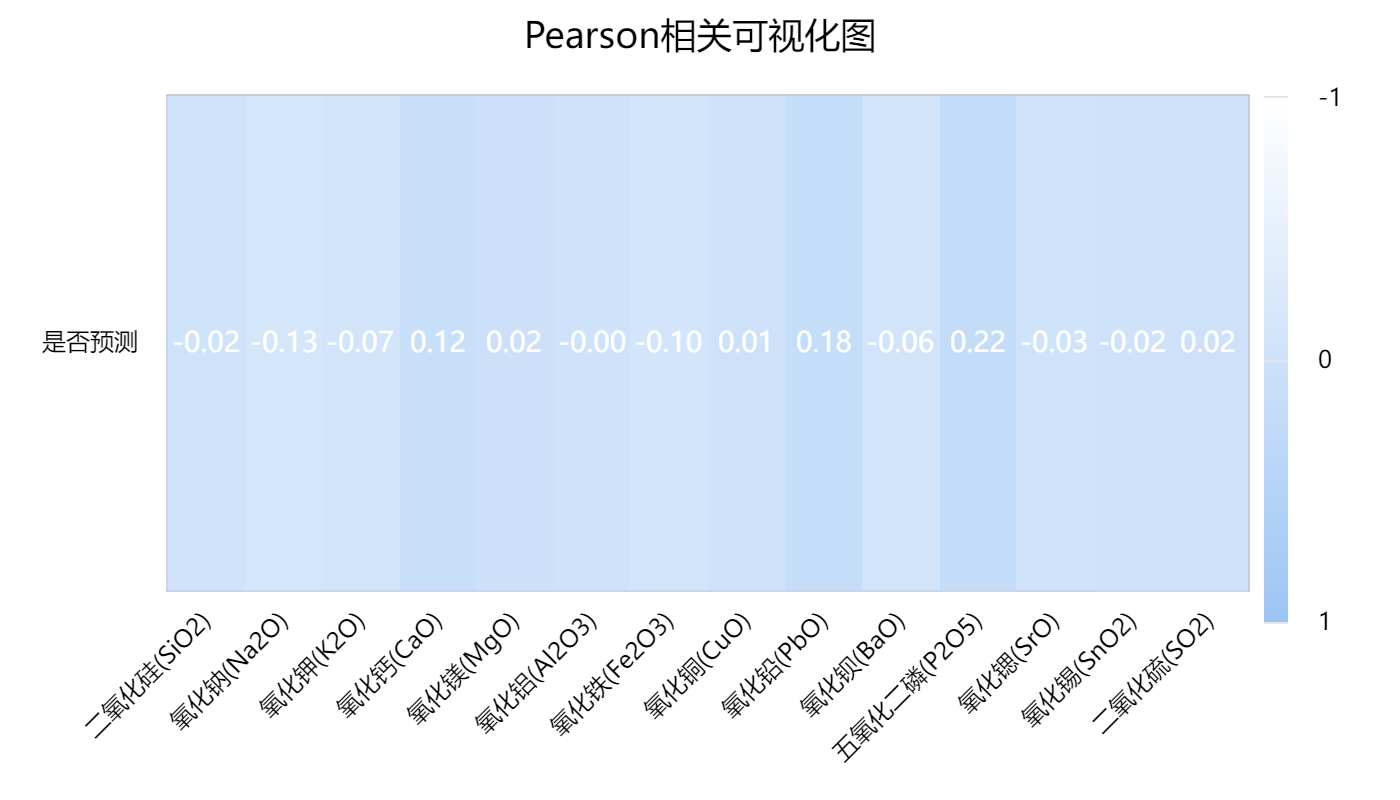
\includegraphics[width=\textwidth]{Bpearson.png}  %设置图片的输出大小倍数,这里是0.5倍大小输出
    \end{minipage}
    }
    \subfigure[高钾玻璃]{ %第二张子图
    \begin{minipage}{0.4\textwidth}
    \centering    %子图居中
    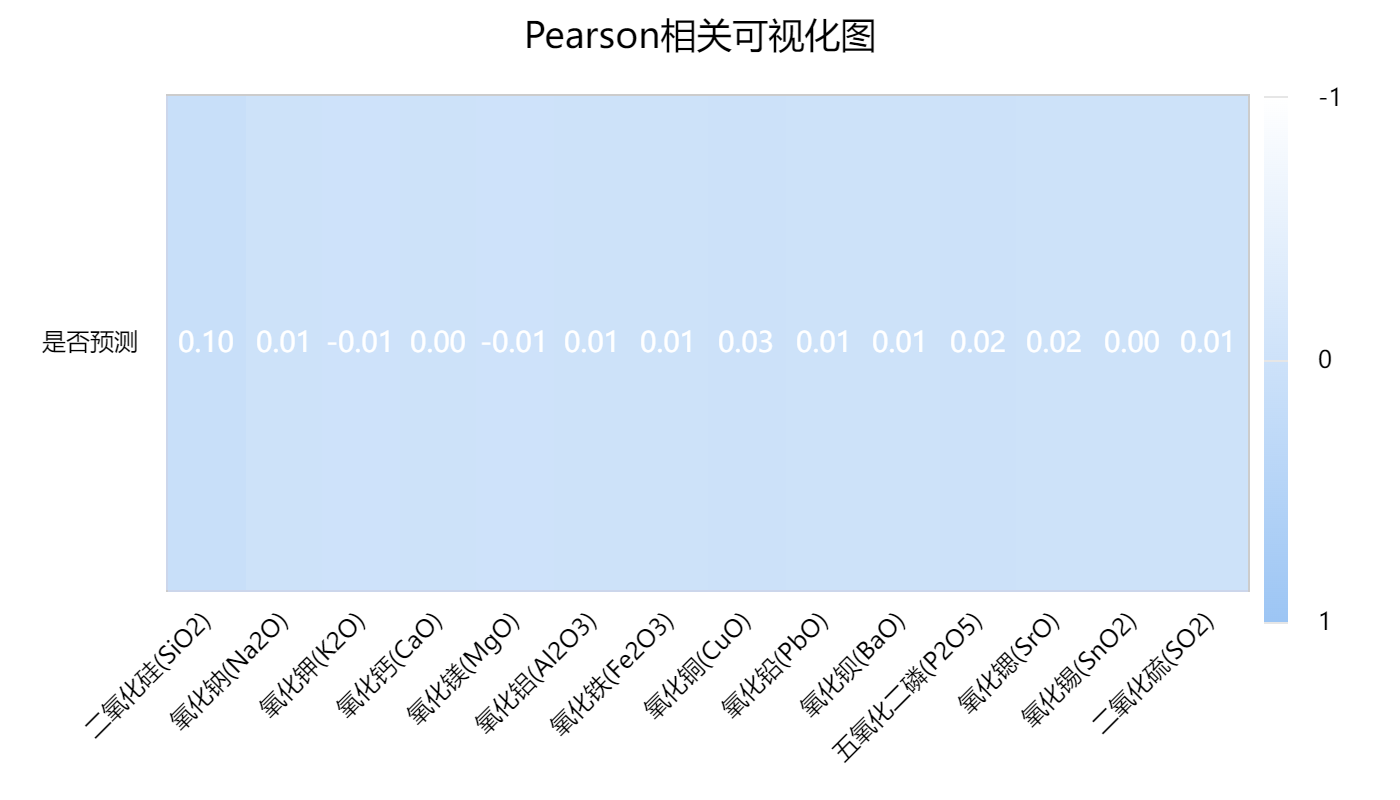
\includegraphics[width=\textwidth]{kpearson.png}%以pic.jpg的0.5倍大小输出
    \end{minipage}
    }
    

    \caption{不同种类玻璃成分同预测之间的相关系数结果}    %大图名称
    \label{pear}    %图片引用标记
\end{figure}
可知各化学成分占比同是否预测之间相关系数值$ p $均大于0.05说明没有相关性,也就验证了我们的预测方法是行之有效的。

\subsection{古代玻璃类型及亚类划分模型}
在本部分我们需要解决古代玻璃的类型划分问题,即给出铅钡玻璃和高钾玻璃之间的分类关系;在这一基础上,要对两种玻璃进一步划更细的亚类,并做敏感性分析,解释其合理性。针对大类划分模型,利用问题1种得到预测风化前的样本数据,统计高钾玻璃与铅钡玻璃间各个化学元素的分界点,以投票方式决定一个样本的种类。

针对亚类划分问题,使用相关文献的知识以及变异系数,挑选重要指标,使用kmeans++聚类方法,利用相关系数确定最佳类中心数目。在得出聚类结果后,对原始数据的化学组成变化进行敏感度分析。

\subsubsection{古代玻璃大类划分模型}
古代玻璃的类型不同,是由于其在制造过程种添加了不同的助熔剂,导致其化学成分有所差异,这是我们进行分类的依据所在。考虑到样本风化后带来相关元素的流失,可能会带来误判,因此利用风化后的数据条目预测其风化前的化学成分比例,利用预测结果进行分类。

我们根据指标$c_{ij}$的与划分界限$h_j$相对大小,判断玻璃在这一指标上倾向于哪一类$v_j$。确定划分界限$ h_j $的方法根据该指标在不同大类下的分布差异而有所不同。我们在图(\ref{hj})中给出化学成分按类别的分布情况,并使用不同颜色标注了类别。
\begin {figure}[h]
\centering % 居中显示
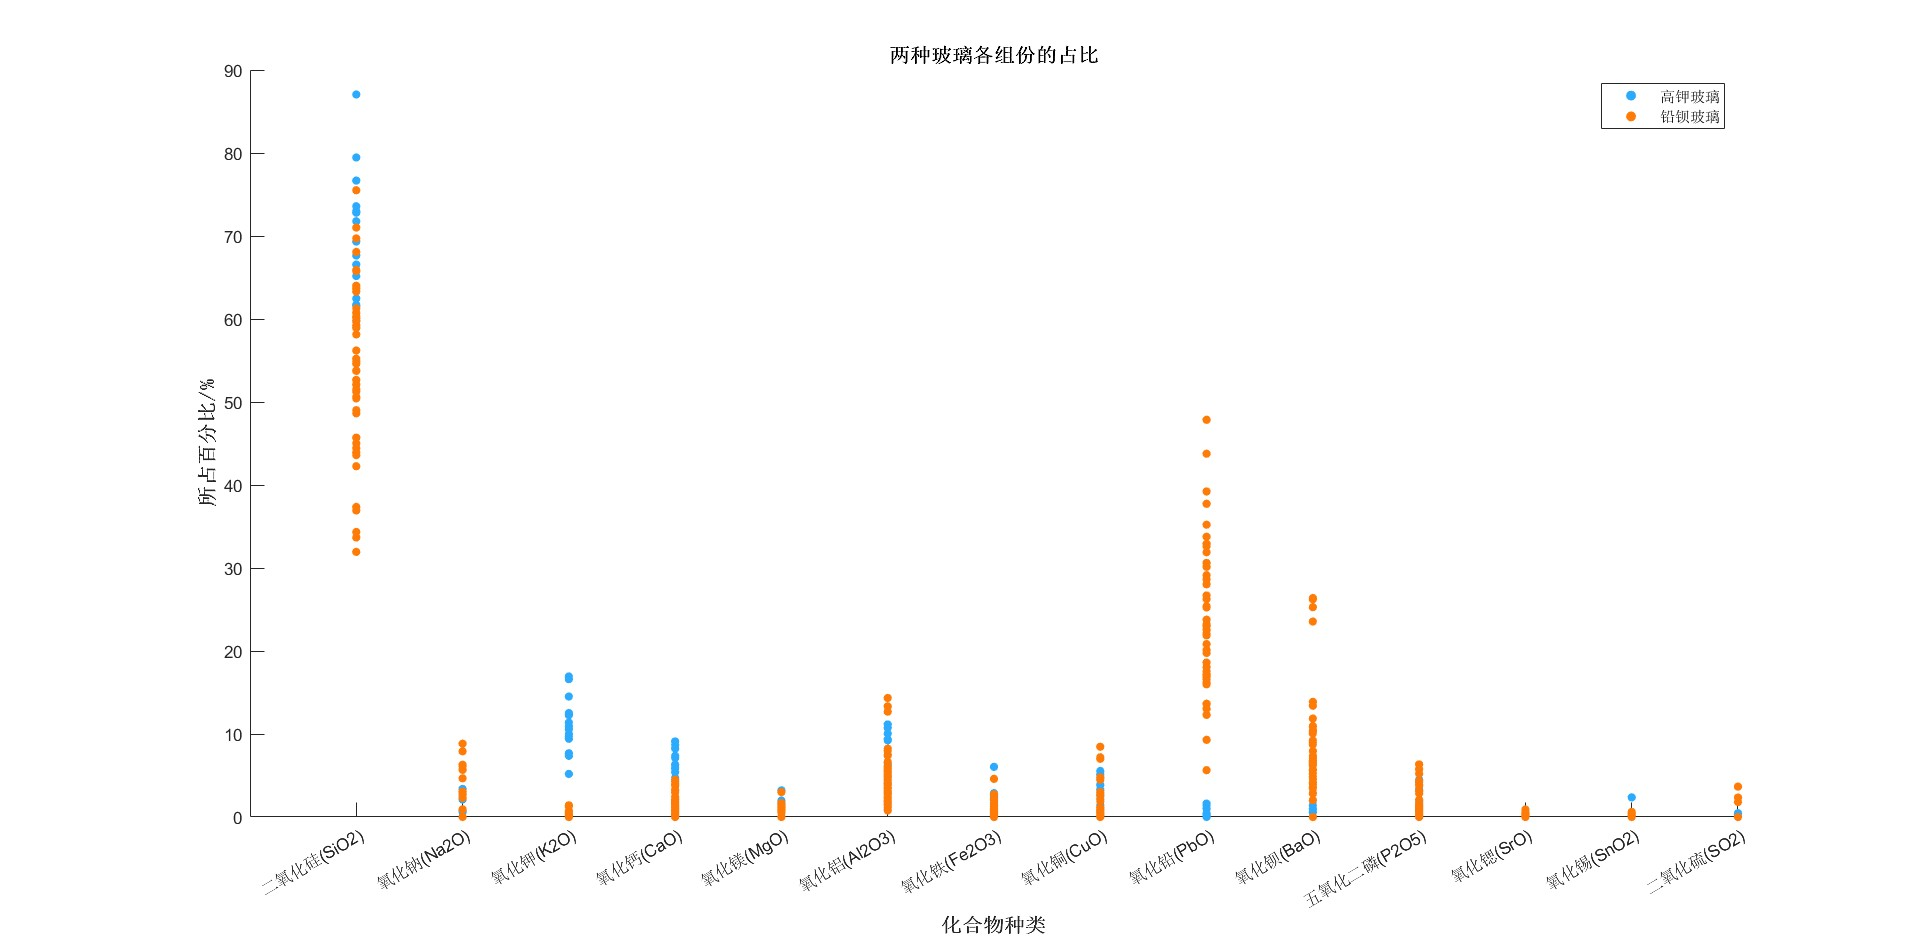
\includegraphics[width=\textwidth]{hj.jpg}
\caption{两种玻璃各个组分的占比} % 标题
\label{hj}
\end {figure}
分析图象可知,部分指标在不同类间具有明显差异,均值较低一类的指标最大值小于另一类该指标的最小值,二者间有明显分界,如氧化钾、氧化钙、氧化铅和氧化锡等。其余指标虽然类之间没有明显间隔,但是仍体现出相对的大小规律。

针对组分占比类间差异的现象,我们灵活给定了划分界限$ h_j $在类间具有明显差异和不明显差异情况下的求解方法。定义$ C_j=\{c_{ij}\,|\,\forall i \,,\, 1\leq i \leq n\} $作为第$ j $个化学成分风化前占比记录的集合,其中$i$是样本序号。$ V=\{v_{i}\,|\,\forall i \,,\, 1\leq i \leq n\} $代表第$i$个指标归属的大类,规定1代表高钾玻璃,0代表铅钡玻璃。

\begin{itemize}
  \item 类间差异明显时
  
  若我们称第$ j $个指标是类间差异明显的,那么指标具有以下关系:
  \begin{equation}
    \begin{cases}
      \underset{v_{a} = 0}{min} \, (c_{aj}) < \underset{v_{b} = 1}{max}\,(c_{bj}) &\,,\, \mu_{0j}<\mu_{1j}\\ 
      \underset{v_{a} = 0}{max} \, (c_{aj}) > \underset{v_{b} = 1}{min}\,(c_{bj}) &\,,\, \mu_{0j}>\mu_{1j}\\ 
    \end{cases}
  \label{diff}
  \end{equation}
  其中$ \mu_0,\mu_1 $分别代表铅钡玻璃和高钾玻璃在第$ j $指标上的均值。在这一条件下,可以给出此时的划分标准$ h_j $:
  \begin{equation}
  h_j=\begin{cases}
    \frac{c_{bj,max}\,+\,c_{aj,min}}{2}&, \mu_{0j}<\mu_{1j}\\
    \frac{c_{bj,min}\,+\,c_{aj,max}}{2}&, \mu_{0j}>\mu_{1j}\\
  \end{cases}
  \label{hj1}
  \end{equation}

  \item 类间差异不明显时
  
  此时两类在同一指标的最大最小值不能满足式(\ref{diff})之间的关系,此时使用两类均值的中点来作为分界$ h_j $:
  \begin{equation}
  h_j = \frac{\mu_{0j}+\mu_{1j}}{2}
  \label{hj2}
  \end{equation}

\end{itemize}

综上,在得到界限$ h_j $后可对第$ i $条记录在第$ j $项成分的上的倾向性$ v_j $进行判断,根据指标同界限$h_j $的相对大小进行倾向划分。

\begin{equation}
v_{ij} =  \begin{cases}
  0 \,,&\, c_{ij}<h_j ,\mu_0<\mu_1 \,,\,\text{或} \,,\, c_{ij}>h_j ,\mu_0>\mu_1 \,\\
  1 \,,&\, c_{ij}<h_j ,\mu_1<\mu_0 \,,\,\text{或} \,,\, c_{ij}>h_j ,\mu_1>\mu_0 \,\\
\end{cases}
\label{vij}
\end{equation}

随后赋权对指标倾向的结果求和,便可得到最终的分类结果。首先计算样本在指标$j$上的均值距离,与样本均值中点的商,并将其归一化后作为权重:
\begin{equation}
D_j = \frac{2*|\mu_{0j}-\mu_{1j}|}{\mu_{0j}+\mu_{1j}}
\label{dj}
\end{equation}
\begin{equation}
w_j = \frac{D_j}{\sum\limits_{j=1}^{14} D_j}
\label{wj}
\end{equation}

最终得到分类函数$ F $,当输出结果大于0.5时认定为高钾玻璃,结果为0时认定为铅钡玻璃。
\begin{equation}
F = \sum\limits_{j=1}^{14} w_j \cdot v_{ij}
\label{F}
\end{equation}

\subsubsection{大类划分模型求解}
我们计算出各指标下的界限值$ h_j $以及对应的权重$w_j$,按权重降序的顺序对化学成分指标进行排列,得到图(\ref{hjtu})
\begin {figure}[h]
\centering % 居中显示
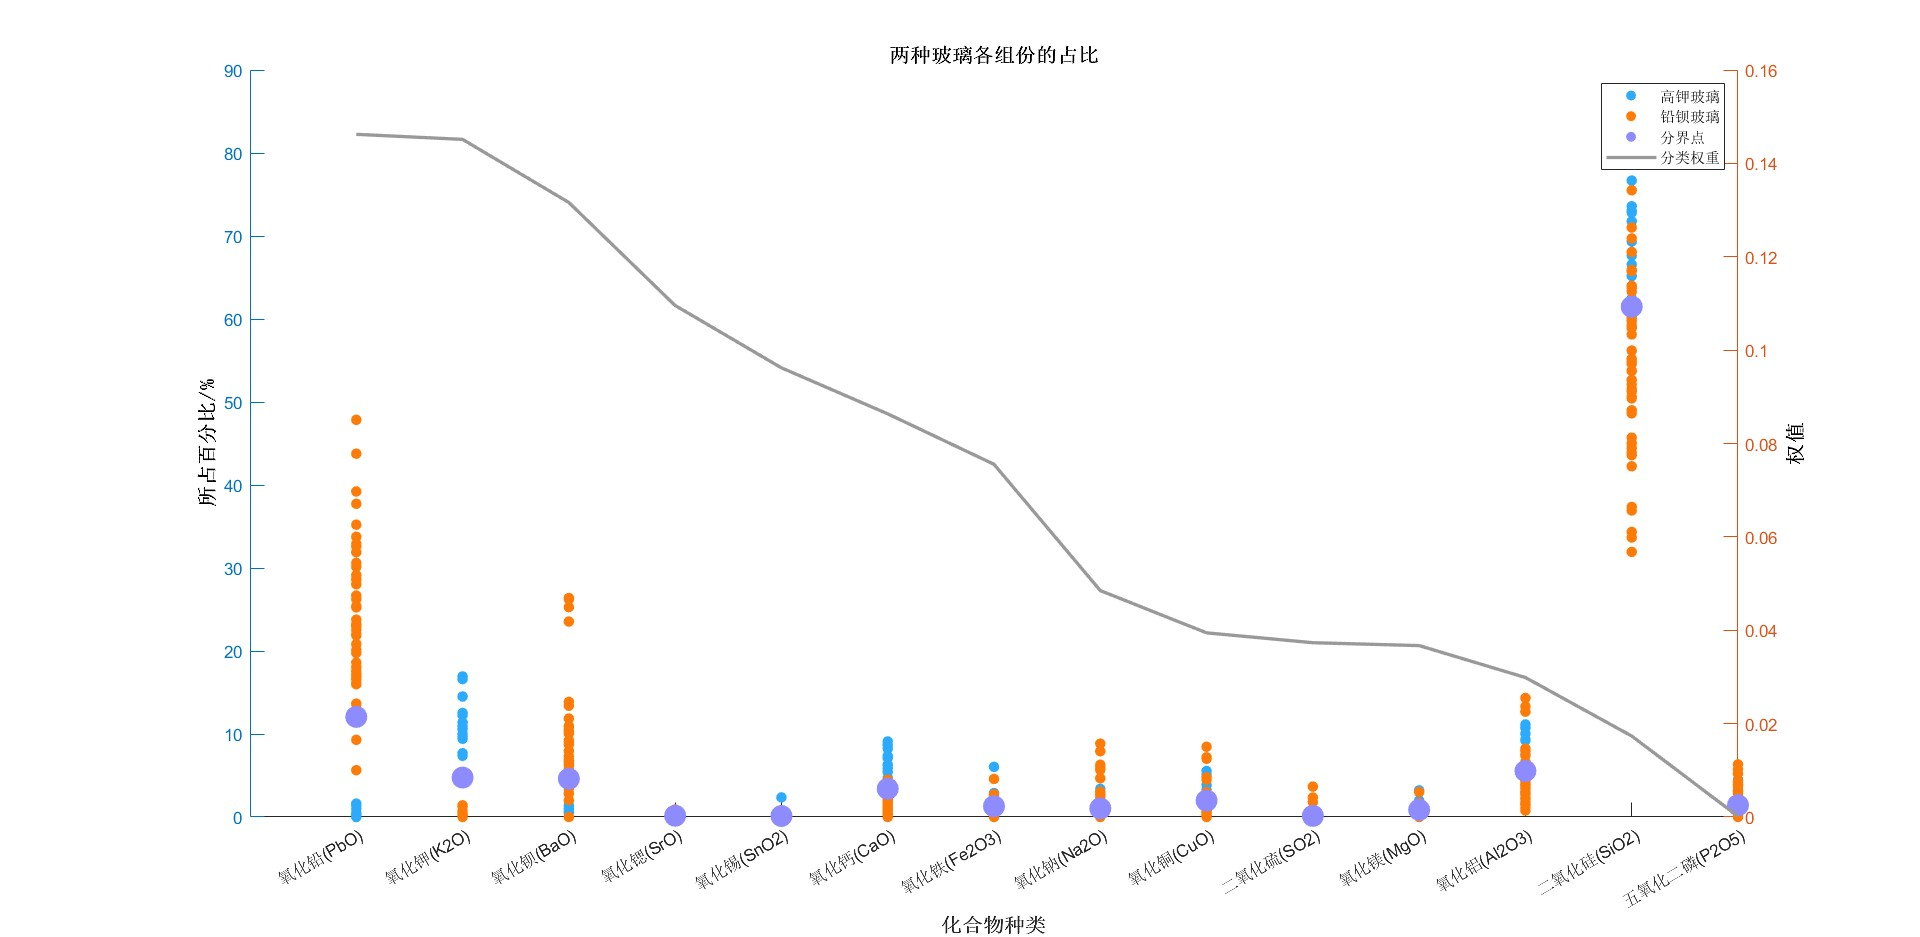
\includegraphics[width=\textwidth]{6.jpg}
\caption{分类指标界限值$ h_j $以及对应的权重$w_j$示意图} % 标题
\label{hjtu}
\end {figure}
\newpage

可见权重较高的前三项成分分别为氧化铅、氧化钾与氧化钡,这是两种玻璃助熔剂差异成分的主要差异,能够支撑分类权重的合理性。对数据混杂,区分不大的指标权重较小,如二氧化硅作为玻璃的主要成分,不具有特殊性,且由于含量的变化范围大,不能显著区分两类玻璃的情况。

在分类的准确性上,我们利用64条数据进行分类测试,高钾玻璃18项全部分类正确,46项铅钡玻璃仅有一个错误,分类正确率为$ 98.44\% $。

\subsubsection{亚类划分模型}
我们首先进行亚类指标筛选。查阅相关资料,一些文献\cite{8,9}常常基于相对丰度的大小,进行亚类的细分。这一划分方式以某一指标的绝对含量进行分析,满足某个条件时便属于某类玻璃。但由于古代玻璃制作工艺的特性,这些指标可能仅对特定地区的玻璃样品具有意义。

因此我们仅参考上述文献所提及的成分指标,包括Na、Al、Ca、Cu、Fe等元素。此外,利用在5.3中给出的统计规律数据,通过变异系数$c_v$筛选出变化幅度较大的若干指标作为聚类指标。考虑到均值过小时变异系数产生异常,对含量均值小于$1\%$的指标也不予考虑。

鉴于在区分高钾玻璃和铅钡玻璃的过程中,氧化铅、氧化钾和氧化钡发挥主要作用,在亚类分析时可不考虑上述三个因素;又因为二氧化硅所占据的成分比例远高于其余成分,会影响其余指标的距离计算,也同样不考虑这一因素。
\newpage
% \begin{figure}[htbp]
%     \
%     \caption{变异系数统计}    %大图名称
%     \label{cvpr}    %图片引用标记
% \end{figure}
\begin {figure}[h]
\centering % 居中显示
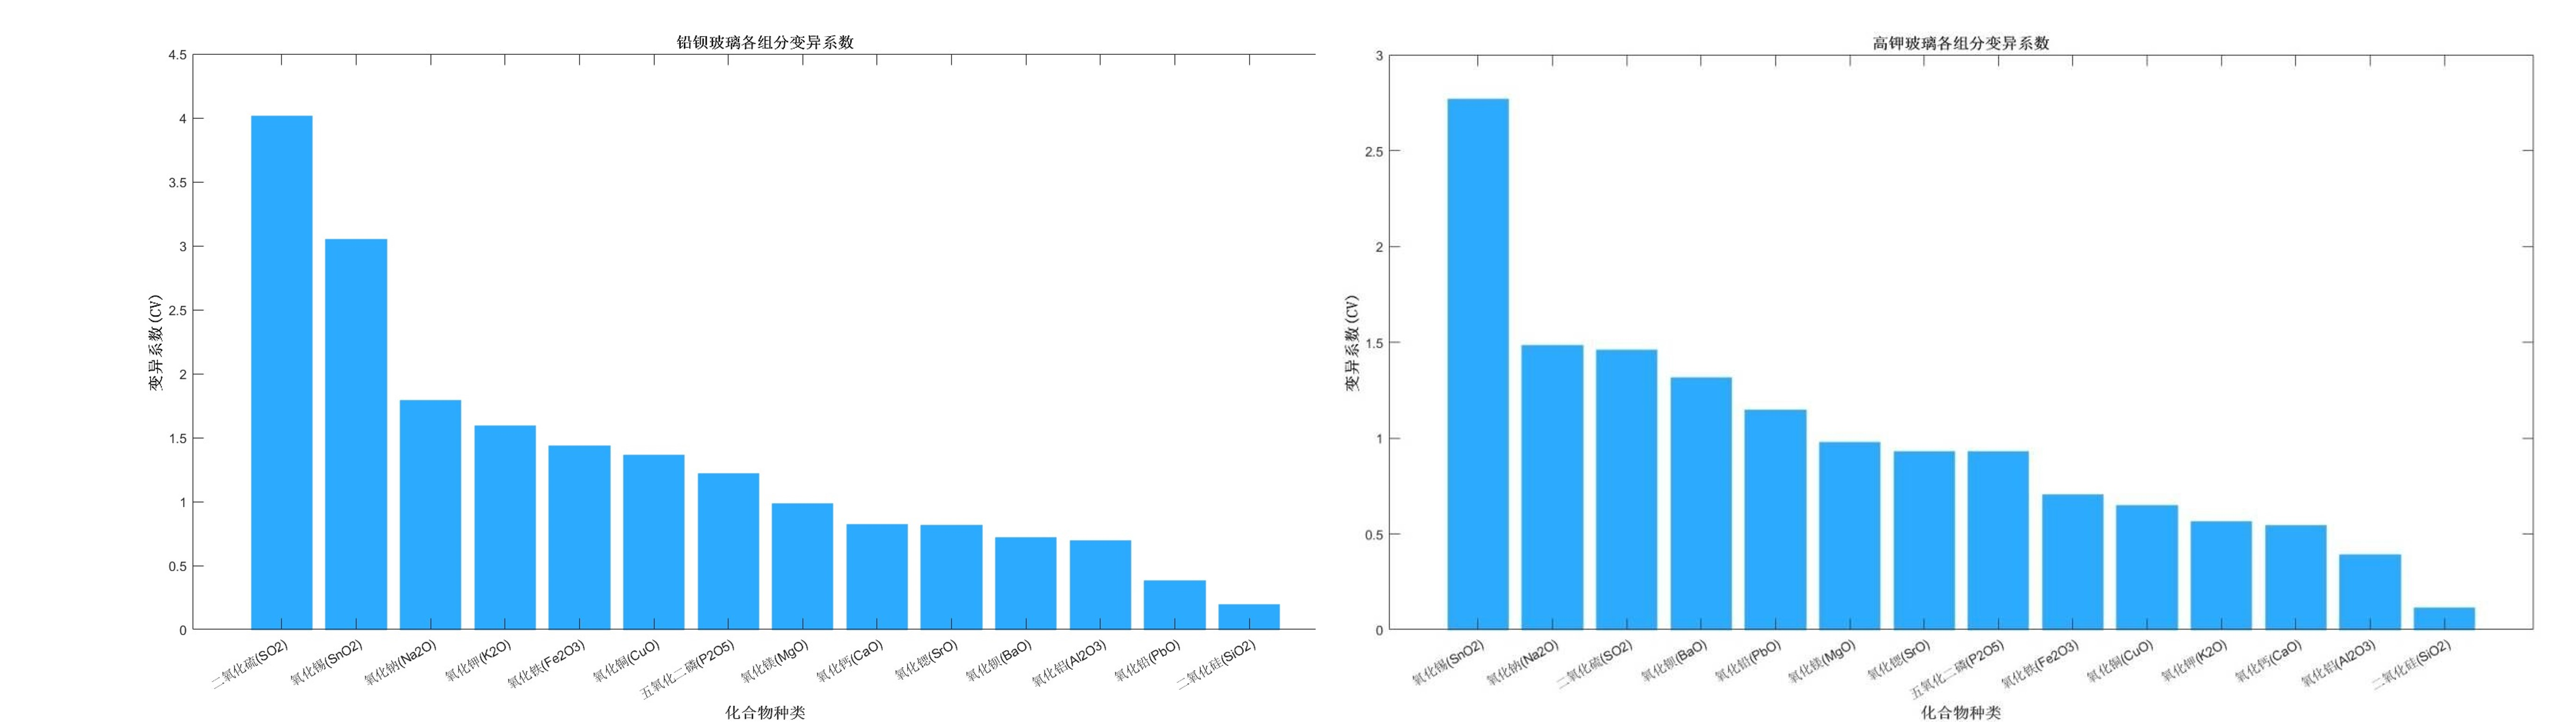
\includegraphics[width=\textwidth]{12.jpg}
\caption{变异系数统计} % 标题
\label{cvpr}
\end {figure}
经过上述分析,最终确定高钾玻璃的亚类划分指标为氧化铝、氧化钙、氧化铜、氧化铁。铅钡玻璃的划分指标为氧化铝、氧化钙、氧化铜、五氧化二磷和氧化钠。均为五项指标。

在筛选重要指标后进行聚类,使用kmeans++算法\cite{10}进行聚类。该算法的基本步骤如下:
\begin{enumerate}
  \item 选择$k$个样本中心,这里的样本指的是原始样本在亚类划分指标上的投影。kmeans++算法优化了该步骤选择初始样本点的过程,达到了更快的收敛速度。\cite{11}
  \item 计算所有样本点到类中心的距离,也就是各个划分指标$c_{ij}$同中心$\bar{c_{k}}$的欧氏距离。
  \item 将样本点分配给最近的类中心所属的类别,也就是更新亚类划分。
  \item 计算每个亚类各项化学成分的均值$\bar{c_k}$。
  \item 重复2-4步,直至各个样本分类的结果保持不变。
\end{enumerate}

使用k均值聚类算法的一大问题在于确定类别的数目$k$,为此,我们使用元素含量同类别之间的F检验相关系数\cite{12}的显著性作为评判标准。这是由于如果分类具有区分度的话,元素含量就可能同分类的结果具有相关性。显然,太少的类别数量不能够有效区分指标间的差异,而过多的分类数量会带来过拟合的问题。随着分类数量的上升,含量同类别的相关系数将会呈现先增加后减少的趋势,选择相关系数之和最小时的k值作为最佳聚类数目。

\subsubsection{亚类划分模型求解}
首先确定聚类的数目,根据不同类型的玻璃分别列表分析最佳聚类数目。针对铅钡玻璃和高钾玻璃的最佳聚类数,列出表(\ref{kb},\ref{kk})。
\begin{longtable}{ccccccc}
\caption{铅钡玻璃聚类数同显著性指标关系表}
\label{kb} \\
\toprule
类数 & 氧化铝 & 氧化钙   & 氧化铜   & 五氧化二磷 & 氧化钠   & 显著性指标和 \\\midrule
2  & 0   & 0.004 & 0.279 & 0     & 0.074 & 0.357  \\
3  & 0   & 0.057 & 0.611 & 0.038 & 0     & 0.706  \\
4  & 0   & 0     & 0.412 & 0     & 0     & 0.412  \\
5  & 0   & 0.032 & 0     & 0     & 0     & 0.032  \\
6  & 0   & 0.005 & 0     & 0     & 0     & 0.005  \\
7  & 0   & 0.004 & 0     & 0     & 0     & 0.004  \\
8  & 0   & 0     & 0     & 0     & 0     & 0      \\
9  & 0   & 0     & 0     & 0     & 0     & 0      \\
\bottomrule
\end{longtable}  

\begin{longtable}{ccccccc}
  \caption{高钾玻璃聚类数同显著性指标关系表}
  \label{kk} \\
  \toprule
  分类数 & 氧化钙 & 氧化铝   & 氧化铜   & 氧化铁   & 五氧化二磷 & 显著性指标和 \\\midrule
2   & 0   & 0.08  & 0.107 & 0.327 & 0.935 & 1.449  \\
3   & 0   & 0.001 & 0.21  & 0.022 & 0     & 0.233  \\
4   & 0   & 0     & 0.006 & 0.013 & 0.001 & 0.02   \\
5   & 0   & 0     & 0.006 & 0     & 0.002 & 0.008  \\
6   & 0   & 0     & 0.009 & 0.001 & 0.001 & 0.011  \\
7   & 0   & 0     & 0.01  & 0.005 & 0.006 & 0.021  \\
8   & 0   & 0     & 0.006 & 0.025 & 0.003 & 0.034  \\
9   & 0   & 0     & 0     & 0.026 & 0.001 & 0.027  \\
  \bottomrule
  \end{longtable}  
\begin{center}
  注:数值为0代表显著性非常强,数值太小向下溢出
\end{center}

最终选定所有指标恰好都满足显著性关系的k值,分别是$k_B = 6\,,\,k_K = 5$。观察表中结果,铅钡玻璃分类后随着类别的增加,显著性指标极强,反映出聚类数量太多导致过拟合。

在此条件下进行聚类,在给定$k$值下进行聚类,得到以下结果:
\begin {figure}[h]
\centering % 居中显示
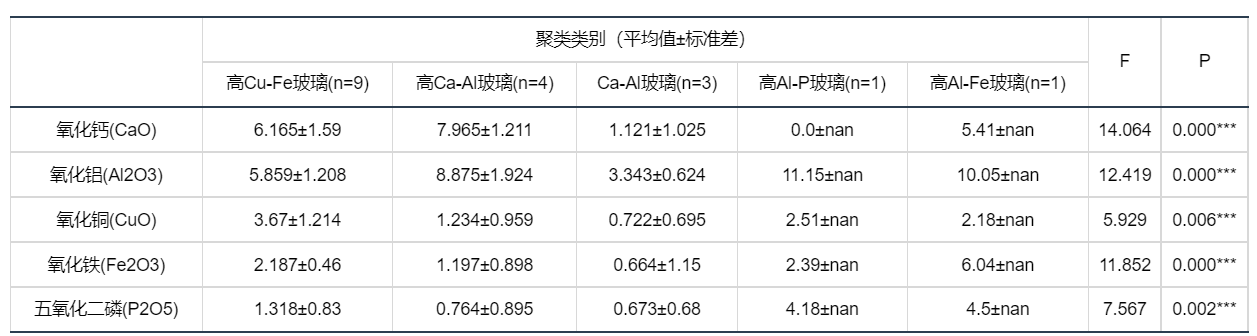
\includegraphics[width=\textwidth]{kkres.png}
\caption{高钾玻璃亚类划分结果} % 标题
\label{kkres}
\end {figure}
\begin {figure}[h]
\centering % 居中显示
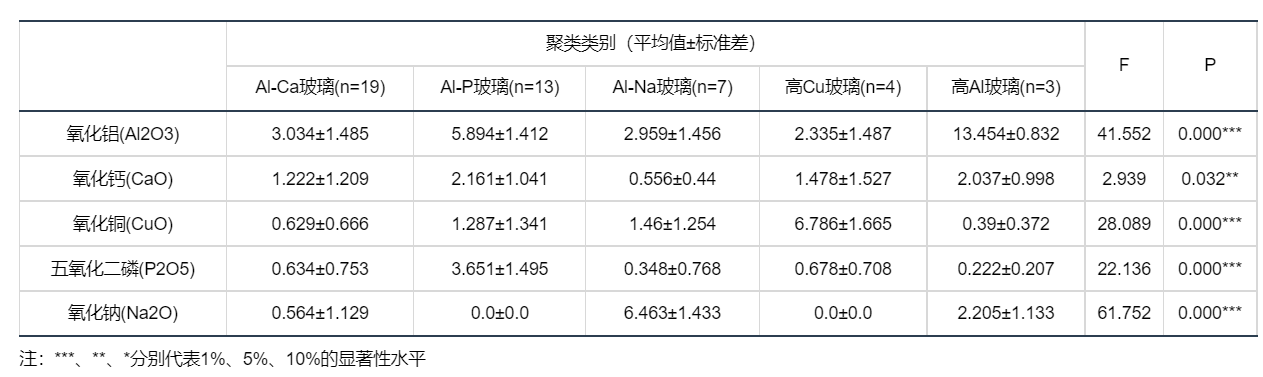
\includegraphics[width=\textwidth]{kbres.png}
\caption{铅钡玻璃亚类划分结果} % 标题
\label{kbres}
\end {figure}

\newpage
我们最终将高钾玻璃划分为\textcolor{red}{亚类成分}分析聚类结果(图\ref{kkres}、图\ref{kbres})可知,每类样本的数量分布都较为合理,且各组分含量的显著性都非常高。我们将利用该划分模型解决问题三,并在6.1中分析亚类划分的敏感性。

\subsection{未知类别文物样本的分类}

对于未知样本的分类问题,可以将其转化为两个子问题,其一是确定样本所属类别,即:属于铅钡玻璃还是高钾玻璃。再对具体哪一个细类进行划分。

为了确定样本归属类别,首先使用5.4中的风化前情况预测模型来预测其风化前的元素含量。利用式(\ref{cijk})以及表(\ref{bianhua})中的数据,得到风化前的化学成分数据。这里使用变化幅度最小的综合变化系数对风化前的样本含量进行预测。
$$    c_{ij}^k = \begin{cases}
  (1+\Delta_{K0})*c_{ij}^k&\,,k=K\\
  (1+\Delta_{B0})*c_{ij}^k&\,,k=B\\
\end{cases} \, \quad , \quad (c_{ij}>0\quad ,\Delta_0 > 0)$$

随后利用5.5.1中给出的大类划分模型(式\ref{F}),对样本的所属种类进行划分。
$$F = \sum\limits_{j=1}^{14} w_j \cdot v_{ij}$$

为了划分亚类,使用5.5.4中给出亚类的中心进行判断,并且计算哪一类的中心距离最近,待分类数据便归属于哪一类。

经由上述步骤,我们给出待分类数据的分类结果,如表(\ref{class})所示。

\begin{longtable}{cccc}
  \caption{未知玻璃样品的类别划分结果}
  \label{class} \\
  \toprule
  文物编号 & 表面风化 & 玻璃类型 & 玻璃亚类     \\\midrule
  A1   & 无风化  & 高钾玻璃 & 高Cu-Fe玻璃 \\
  A2   & 风化   & 铅钡玻璃 & Al-P玻璃   \\
  A3   & 无风化  & 铅钡玻璃 & Al-P玻璃   \\
  A4   & 无风化  & 铅钡玻璃 & Al-P玻璃   \\
  A5   & 风化   & 铅钡玻璃 & 高Al玻璃    \\
  A6   & 风化   & 高钾玻璃 & 高Cu-Fe玻璃  \\
  A7   & 风化   & 高钾玻璃 & 高Ca-Al玻璃  \\
  A8   & 无风化  & 铅钡玻璃 & 高Cu玻璃    \\
  \bottomrule
  \end{longtable}  

\subsection{各类玻璃成分关联关系分析模型}
\subsubsection{各类玻璃成分相关程度的确定}
我们选用皮尔逊相关系数和最大信息系数来同时对各个成分的相关性进行衡量。皮尔逊系数可以很好的衡量两随机变量之间的线性相关性,但有些变量具有很强的非线性相关性,其皮尔逊相关系数却很低,所以我们又使用了最大信息系数。互信息可以衡量一个随机变量中包含的关于另一个随机变量的信息量。对于两个随机变量的散点图而言,存在某种网格覆盖散点图;根据各散点在网格中子格内的频率来计算变量之间的相关系数。因此其对线性和非线性关性都有很好的度量效果。

互信息\cite{13}的概念使用以下方程来说明:

$$I(x ; y)=\int p(x, y) \log _{2} \frac{p(x, y)}{p(x) p(y)} \mathrm{d} x \mathrm{~d} y$$
$$ I[x ; y] \approx I[X ; Y]=\sum_{X, Y} p(X, Y) \log _{2} \frac{p(X, Y)}{p(X) p(Y)}$$

$p(x,y)$为变量x和y之间的联合概率,一般情况下联合概率计算相对来说比较麻烦。

MIC \cite{14}的想法是针对两个变量之间的关系,将其离散在二维空间中,并且使用散点图来表示,将当前二维空间在 x,y 方向分别划分为一定的区间数,然后查看当前的散点在各个方格中落入的情况,这就是联合概率的计算,这样就解决了在互信息中的联合概率难求的问题。下面的公式给出 MIC 的计算公式:

$$\operatorname{mic}(x ; y)=\max _{a * b<B} \frac{I(x ; y)}{\log _{2} \min (a, b)}$$
$$M I C[x ; y]=\max _{|X \| Y|<B} \frac{I[X ; Y]}{\log _{2}(\min (|X|,|Y|))}$$

上式中 a,b 是在 x,y 方向上的划分格子的个数,本质上就是网格分布,B 是变量,在原作者的论文当中提到 B 的大小设置是数据量的 0.6 次方左右。

实际编程时我们直接调用python中的minepy包,将每类玻璃中的各个成分两两组合输入函数来求解。由于最大信息熵在样本量较小的情况下会有些许误差,所以我们同时也做了皮尔逊相关系数的计算来辅助判断关联关系。

最终得到相关系数矩阵(仅以高钾玻璃未风化为例):

\begin {figure}[h]
\centering % 居中显示
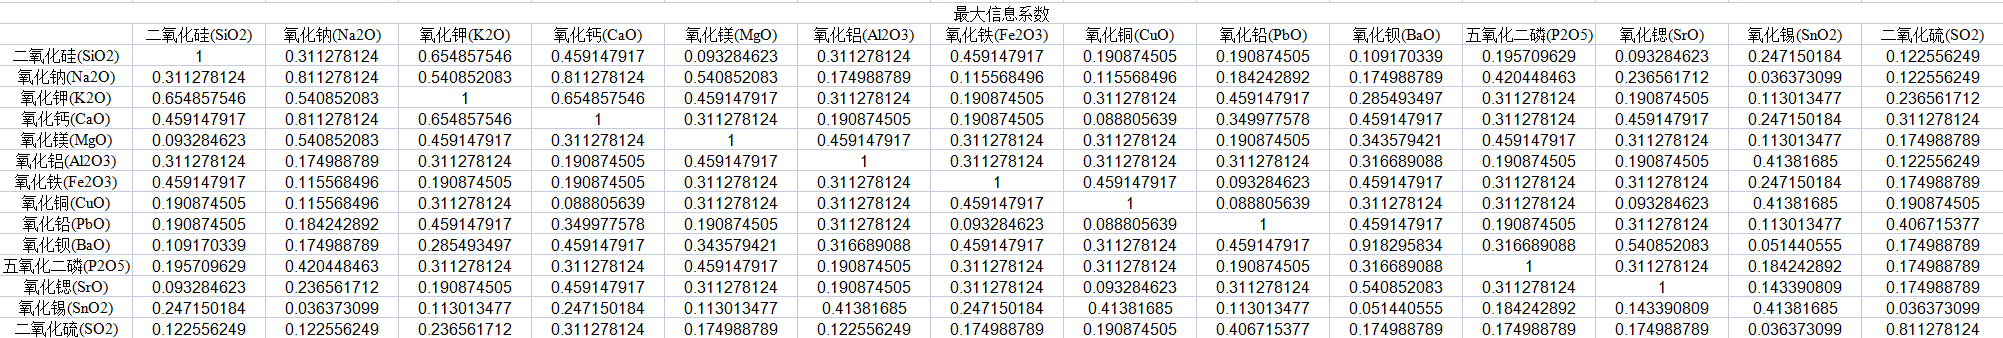
\includegraphics[width=\textwidth]{st1.png}
\caption{相关系数矩阵(部分1)} % 标题
\label{five}
\end {figure}
\begin {figure}[h]
\centering % 居中显示
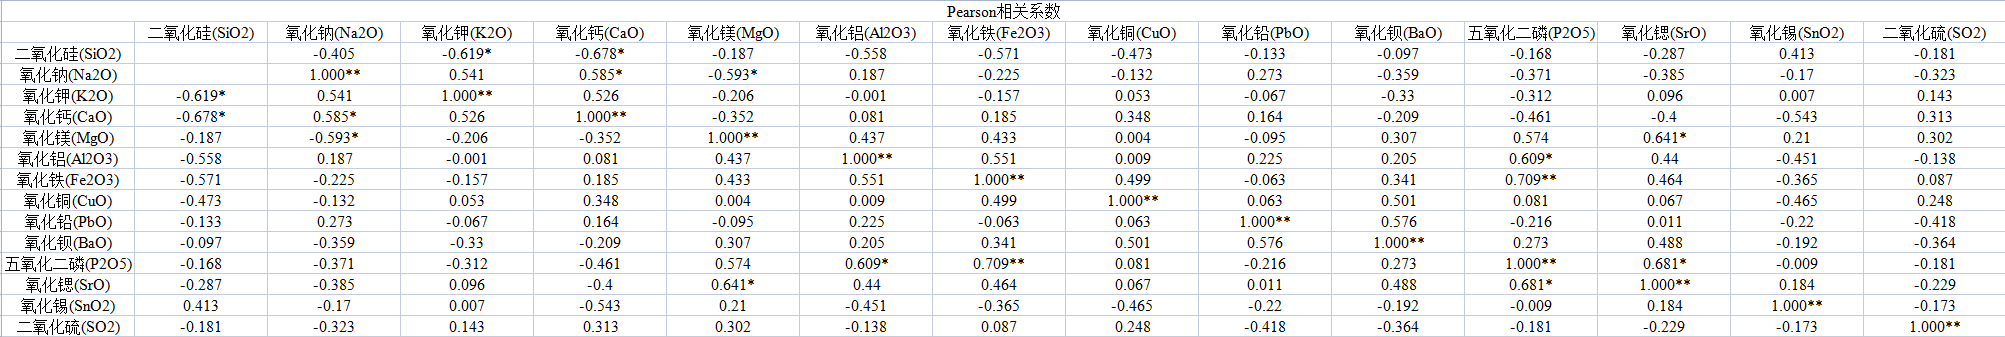
\includegraphics[width=\textwidth]{st2.png}
\caption{相关系数矩阵(部分2)} % 标题
\label{five}
\end {figure}

\subsubsection{各类型玻璃两两成份之间关系的确定}

由于样本数量较小,所以有些指标与其自身的最大信息系数不为1,在所有相关系数矩阵中,自身的最大信息系数最小为0.4,所以我们挑选最大信息系数超过0.4的成分组合做各种函数的拟合。

我们选择最常见的其中函数作为拟合目标,分别为:幂函数、指数函数 、双曲线函数 、对数函数 、指数函数 、S型曲线 和一次函数y=kx+b。拟合使用matlab自带的nlifit来拟合。初始点的选取对拟合效果有较大影响,我们选取与未知系数相同数量的原始数据点数,代入方程求解出一组系数,做为初始系数,这样系数的数量级和数量关系是可以大体确定的。对于某些数据点,我们无法对其作相关函数的拟合尝试,比如y = ln(x)不可对x=0的数据点进行拟合,我们便舍弃此函数。

拟合后我们利用R-square来衡量每种拟合方式的拟合效果,最终选取拟合优度最高的 拟和函数作为两成份的定量关系。现以相关性较强的两组指标为例展示。

\begin {figure}[h]
\centering % 居中显示
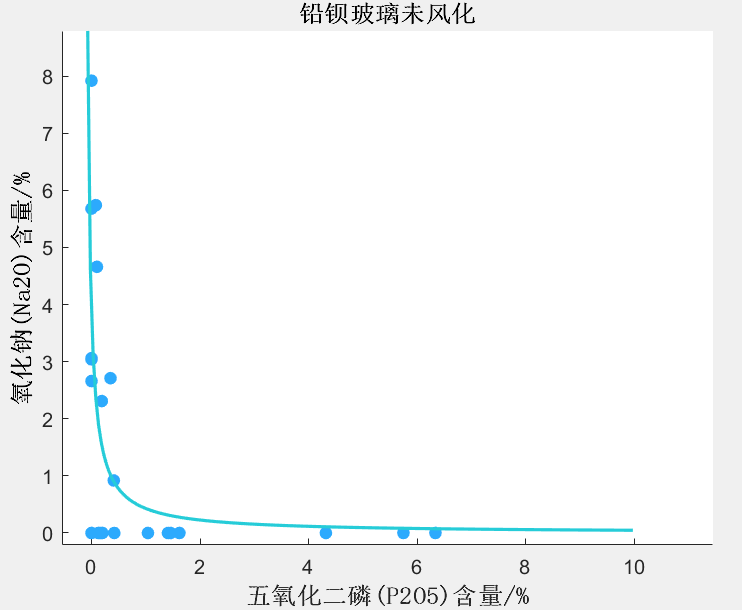
\includegraphics[width=0.7\textwidth]{st3.png}
\caption{氧化钠同五氧化二磷关系} % 标题
\label{five}
\end {figure}

R-square = 0.4202;拟合关系式:y = 1/(0.2586 + 2.0735x);

分析:铅钡玻璃未风化类别中,五氧化二磷和大致成反比例关系,即要么两者都少,要么一个多,另一个必然少。

\begin {figure}[h]
\centering % 居中显示
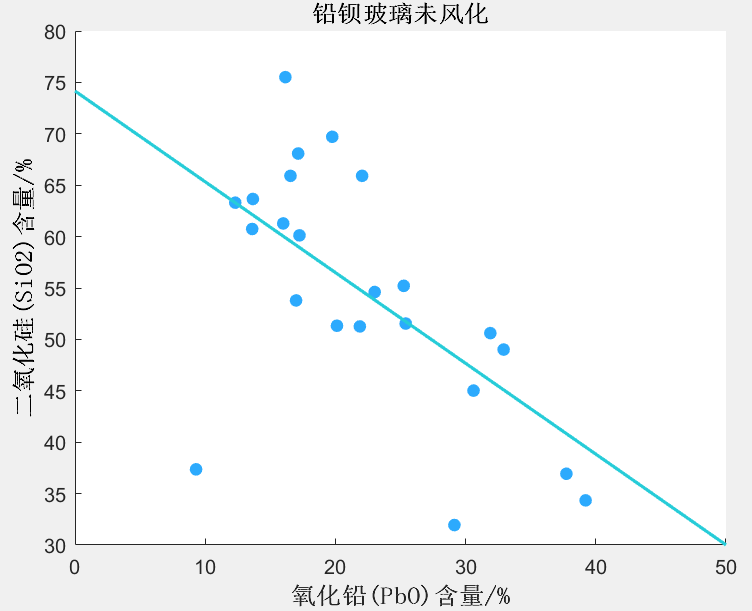
\includegraphics[width=0.7\textwidth]{st4.png}
\caption{氧化铅同二氧化硅关系} % 标题
\label{five}
\end {figure}

square = 0.3761;拟合关系式:y = 74.1619 - 0.8831x;

分析:铅钡玻璃中二氧化硅和氧化铅成反比关系,因为而这都是这种玻璃的主要元素,所以一个含量增加时,会导致另一个含量下降。

\subsubsection{多个成分相关性量化分析}

我们通过皮尔逊相关系数矩阵,可以发现有几个指标具有相互连接的较高的线性相关度,如氧化钾与二氧化硅,二氧化硅与氧化钙,氧化钙与氧化纳,氧化钠与氧化镁,他们都具有较显著的线性相关性。所以我们尝试对这几个成分进行多元线性拟合,并分析其复相关系数。观察多个成分之间的关系。

多元线性拟合得到:C(氧化纳) =4.856 - 1.4151*C(氧化钾)-0.049673*C(二氧化硅)-0.65879*C(氧化钙)+1.1259C(氧化镁)

分析:其复相关系数虽然不如其中参与元素两两之间的皮尔逊系数大,但是与成分两两组合的R-square相当,所以此多元线性拟合还是能够反映一定规律的。由关系式知氧化纳与氧化钾、二氧化硅和氧化钙成反比,而与氧化镁成正比。

\section{六、敏感性分析}
\subsection{亚类划分情况的敏感性分析}
在5.5中,我们提出一种基于k-means聚类的亚类划分模型,亚类的数据来源是综合资料和数据特点选出的若干主要化学成分。由于古代玻璃的制造工艺特性,一个样本各处的含量可能有所差异,因此会对聚类结果造成影响。为了探究对于原始数据波动带来的影响,使用分类正确率的变化衡量模型的敏感性。

在每次测试中,我们对某一指标进行一定幅度的变动,记录变动过后分类的正确性,由表(\ref{senk},\ref{senb})给出。

\begin{longtable}{cccccc}
\caption{铅钡玻璃亚类划分敏感性分析}
\label{senb} \\
\toprule
& 氧化铝(Al2O3) & 氧化钙(CaO) & 氧化铜(CuO) & 五氧化二磷(P2O5) & 氧化钠(Na2O) \\\midrule
10\%  & 95.65\%    & 95.65\%  & 93.48\%  & 95.65\%     & 95.65\%   \\
5\%   & 100\%      & 95.65\%  & 97.83\%  & 97.83\%     & 97.83\%   \\
-5\%  & 97.83\%    & 93.48\%  & 95.65\%  & 97.83\%     & 100\%     \\
-10\% & 97.83\%    & 97.83\%  & 93.48\%  & 93.48\%     & 95.65\%   \\
\bottomrule
\end{longtable}  

\begin{longtable}{cccccc}
  \caption{高钾玻璃亚类划分敏感性分析}
  \label{senk} \\
  \toprule
  & 氧化钙 & 氧化铝   & 氧化铜   & 氧化铁   & 五氧化二磷 \\\midrule
  10\%  & 72.22\% & 66.67\% & 83.33\% & 66.67\% & 83.33\% \\
  5\%   & 83.33\% & 72.22\% & 88.89\% & 72.22\% & 83.33\% \\
  -5\%  & 88.89\% & 77.78\% & 94.44\% & 83.33\% & 88.89\% \\
  -10\% & 77.78\% & 66.67\% & 77.78\% & 72.22\% & 77.78\% \\
  \bottomrule
  \end{longtable} 

可见铅钡玻璃在数据波动时其稳定性较好,最坏情况下也能达到$93.48\%$的分类准确性,而高钾玻璃稳定性欠佳,最坏情况下有约三分之一的数据不能正确分类。出现这一结果得到原因在于二者样本量的数量有差距,铅钡玻璃这一大类具有46项数据,而高钾玻璃大类仅有18项数据,这一定程度上影响了稳定性。另外,一些指标由于其较大的含量占比,波动时容易盖过其余指标的权值,导致分类时产生错误,这是不同数据相同幅度,带来不同结果的原因。

\subsection{未知样本预测的敏感性分析}

\subsubsection{大类敏感性分析}
要分析未知样本的大类敏感性,我们对5.5.1中提出的划分标准$h_j$数值分别浮动一定程度,观察分类结果的正确性变化。得出表(\ref{sen2})
\begin{longtable}{ccccc}
\caption{预测模型大类敏感性结果}
\label{sen2} \\
\toprule
& 氧化钾(K2O) & 氧化铅(PbO) & 氧化钡(BaO) & 氧化锶(SrO) \\\midrule
10\%  & 100\%    & 87.50\%  & 87.50\%  & 87.50\%  \\
5\%   & 87.50\%  & 87.50\%  & 100\%    & 100\%    \\
-5\%  & 100\%    & 100\%    & 100\%    & 100\%    \\
-10\% & 87.50\%  & 100\%    & 100\%    & 100\%    \\
\bottomrule
\end{longtable}  
在相关分界有波动时,会导致一些分类错误,对于那些波动后分类准确率不变的成分,我们由于篇幅所限没有展示。在出现波动时正确率小于百分之九十的原因是待预测样本数量太少。

\subsubsection{亚类敏感性分析}
在分析亚类敏感性时,对数据成分进行浮动,对应产生的k-means聚类中心也可能发生变化,分析此时亚类分类的变化情况。得到表(\ref{sen3},\ref{sen4})。
\newpage 
\begin{longtable}{cccccc}
\caption{高钾玻璃亚类分析}
\label{sen3} \\
\toprule
& 氧化钙(CaO) & 氧化铝(Al2O3) & 氧化铜(CuO) & 氧化铁(Fe2O3) & 五氧化二磷(P2O5) \\\midrule
5\%   & 100\%    & 100\%      & 100\%    & 100\%      & 100\%       \\
10\%  & 87.50\%  & 100\%      & 100\%    & 100\%      & 100\%       \\
-10\% & 100\%    & 87.50\%    & 100\%    & 100\%      & 100\%       \\
-5\%  & 100\%    & 100\%      & 100\%    & 100\%      & 100\%       \\
\bottomrule
\end{longtable}  

\begin{longtable}{cccccc}
  \caption{铅钡玻璃亚类分析}
  \label{sen4} \\
  \toprule
  & 氧化铝(Al2O3) & 氧化钙(CaO) & 氧化铜(CuO) & 五氧化二磷(P2O5) & 氧化钠(Na2O) \\\midrule
  5\%   & 100\%      & 100\%    & 100\%    & 100\%       & 100\%     \\
  10\%  & 100\%      & 100\%    & 100\%    & 100\%       & 100\%     \\
  -10\% & 100\%      & 100\%    & 100\%    & 100\%       & 100\%     \\
  -5\%  & 100\%      & 100\%    & 100\%    & 100\%       & 100\%     \\
  15\%  & 87.50\%    & 100\%    & 100\%    & 100\%       & 100\%     \\
  20\%  & 87.50\%    & 100\%    & 100\%    & 100\%       & 100\%     \\
  -20\% & 100\%      & 100\%    & 100\%    & 100\%       & 100\%     \\
  -15\% & 100\%      & 100\%    & 100\%    & 100\%       & 100\%     \\
  \bottomrule
  \end{longtable}  

  由表分析可知亚类的稳定性更好,在数据出现更大范围波动时,错误率没有发生太大变化。
\section{七、模型的评价}

\subsection{模型的优点}
\begin{enumerate}
    \item 在有用参考文献较少的情况下,能够从数据出发,对各个问题做出合理的解决,能够综合利用多种模型和方法,创新性较高。
    \item 在数据量较小的不利情况下,模型的敏感性分析较多,检验方法丰富,提高了模型的可信度。

\end{enumerate}

\subsection{模型的缺点}
\begin{itemize}
    \item 在预测未风化状态时对一些已经流失的数据数据没有合适的处理
    \item 没有有效的利用铅钡玻璃的三个严重风化数据
    \item 聚类时剔除了一些含量较少的指标可能造成亚类的减少
\end{itemize}

%----------- 参考文献 ----------
\newpage
\begin{center}
\bibliography{r} %调出LaTeX生成参考文献列表
\end{center}

%----------- 附录 ----------
\newpage
\section{附件}
\textbf{附件清单:}
\renewcommand\theenumi{\roman{enumi}}
% 规定数字格式为罗马数字
\renewcommand\labelenumi{\textbf{附录\theenumi}}
% 规定是附录某某
\begin{enumerate}
    \item 统计规律分析结果
    \begin{itemize}
        \item 高钾玻璃风化数据统计(表\ref{index2})
        
        \begin{table}[ht]
            \centering
            \caption{风化高钾玻璃统计量}
            \begin{tabular}{cccccccc}
            \toprule
            名称                   & 样本量                 & 最小值                  & 最大值                  & 平均值                 & 标准差                 & 中位数                 & 变异系数(CV)            \\
            \midrule
            二氧化硅(SiO2)           & 6                    & 92.35                & 96.77                & 93.963               & 1.734                & 93.505               & 1.845\%              \\
            氧化钠(Na2O)            & 6                    & 0                    & 0                    & 0                    & 0                    & 0                    & null                 \\
            氧化钾(K2O)             & 6                    & 0                    & 1.01                 & 0.543                & 0.445                & 0.665                & 81.935\%             \\
            氧化钙(CaO)             & 6                    & 0.21                 & 1.66                 & 0.87                 & 0.488                & 0.83                 & 56.066\%             \\
            氧化镁(MgO)             & 6                    & 0                    & 0.64                 & 0.197                & 0.306                & 0                    & 155.752\%            \\
            氧化铝(Al2O3)           & 6                    & 0.81                 & 3.5                  & 1.93                 & 0.964                & 1.72                 & 49.974\%             \\
            氧化铁(Fe2O3)           & 6                    & 0.17                 & 0.35                 & 0.265                & 0.069                & 0.275                & 26.226\%             \\
            氧化铜(CuO)             & 6                    & 0.55                 & 3.24                 & 1.562                & 0.935                & 1.545                & 59.861\%             \\
            氧化铅(PbO)             & 6                    & 0                    & 0                    & 0                    & 0                    & 0                    & null                 \\
            氧化钡(BaO)             & 6                    & 0                    & 0                    & 0                    & 0                    & 0                    & null                 \\
            五氧化二磷(P2O5)          & 6                    & 0                    & 0.61                 & 0.28                 & 0.21                 & 0.28                 & 74.983\%             \\
            氧化锶(SrO)             & 6                    & 0                    & 0                    & 0                    & 0                    & 0                    & null                 \\
            氧化锡(SnO2)            & 6                    & 0                    & 0                    & 0                    & 0                    & 0                    & null                 \\
            二氧化硫(SO2)            & 6                    & 0                    & 0                    & 0                    & 0                    & 0                    & null                 \\
            \bottomrule
              \end{tabular}
            \label{index2}
        
            注:表中除变异系数外的数据单位为百分比($\%$),null代表无法计算变异系数。
              \end{table}
        \item 铅钡玻璃未风化数据统计(表\ref{index3})
        
        \begin{longtable}{cccccccc}
        \caption{未风化铅钡玻璃统计量}
        \label{index3} \\
        \toprule
            名称                   & 样本量                 & 最小值                  & 最大值                  & 平均值                 & 标准差                 & 中位数                 & 变异系数(CV)            \\
            \midrule
            氧化钠(Na2O)            & 23                   & 0                    & 7.92                 & 1.683                & 2.372                & 0                    & 140.950\%            \\
            氧化钾(K2O)             & 23                   & 0                    & 1.41                 & 0.219                & 0.31                 & 0.15                 & 141.778\%            \\
            氧化钙(CaO)             & 23                   & 0                    & 4.49                 & 1.32                 & 1.285                & 0.84                 & 97.294\%             \\
            氧化镁(MgO)             & 23                   & 0                    & 1.67                 & 0.64                 & 0.547                & 0.71                 & 85.372\%             \\
            氧化铝(Al2O3)           & 23                   & 1.42                 & 14.34                & 4.456                & 3.262                & 3.86                 & 73.213\%             \\
            氧化铁(Fe2O3)           & 23                   & 0                    & 4.59                 & 0.737                & 1.155                & 0                    & 156.782\%            \\
            氧化铜(CuO)             & 23                   & 0                    & 8.46                 & 1.432                & 1.97                 & 0.65                 & 137.586\%            \\
            氧化铅(PbO)             & 23                   & 9.3                  & 39.22                & 22.085               & 8.215                & 20.12                & 37.198\%             \\
            氧化钡(BaO)             & 23                   & 2.03                 & 26.23                & 9.002                & 5.825                & 8.99                 & 64.713\%             \\
            五氧化二磷(P2O5)          & 23                   & 0                    & 6.34                 & 1.049                & 1.847                & 0.19                 & 176.056\%            \\
            氧化锶(SrO)             & 23                   & 0                    & 0.91                 & 0.268                & 0.243                & 0.26                 & 90.752\%             \\
            氧化锡(SnO2)            & 23                   & 0                    & 0.44                 & 0.047                & 0.127                & 0                    & 273.714\%            \\
            二氧化硫(SO2)            & 23                   & 0                    & 3.66                 & 0.159                & 0.763                & 0                    & 479.583\%            \\ \bottomrule
        \end{longtable}  
        \begin{center}
          注:表中除变异系数外的数据单位为百分比($\%$),null代表无法计算变异系数。
        \end{center}

    \item 铅钡玻璃风化数据统计(表\ref{index4})
    \begin{longtable}{cccccccc}
    \caption{铅钡玻璃风化数据统计}
    \label{index4} \\
    \toprule
    名称                   & 样本量                 & 最小值                  & 最大值                  & 平均值                 & 标准差                 & 中位数                 & 变异系数(CV)            \\
    \midrule
    二氧化硅(SiO2)           & 23                   & 12.41                & 53.33                & 27.056               & 9.005                & 25.74                & 33.283\%             \\
    氧化钠(Na2O)            & 23                   & 0                    & 2.22                 & 0.244                & 0.587                & 0                    & 240.349\%            \\
    氧化钾(K2O)             & 23                   & 0                    & 1.05                 & 0.133                & 0.246                & 0                    & 184.408\%            \\
    氧化钙(CaO)             & 23                   & 0.37                 & 6.4                  & 2.777                & 1.667                & 2.82                 & 60.007\%             \\
    氧化镁(MgO)             & 23                   & 0                    & 2.73                 & 0.687                & 0.719                & 0.59                 & 104.803\%            \\
    氧化铝(Al2O3)           & 23                   & 0.45                 & 13.65                & 3.099                & 2.747                & 2.51                 & 88.628\%             \\
    氧化铁(Fe2O3)           & 23                   & 0                    & 2.74                 & 0.661                & 0.751                & 0.33                 & 113.615\%            \\
    氧化铜(CuO)             & 23                   & 0                    & 10.57                & 2.221                & 2.981                & 0.88                 & 134.180\%            \\
    氧化铅(PbO)             & 23                   & 15.71                & 70.21                & 43.71                & 12.077               & 44.12                & 27.631\%             \\
    氧化钡(BaO)             & 23                   & 0                    & 32.25                & 10.475               & 7.966                & 8.64                 & 76.048\%             \\
    五氧化二磷(P2O5)          & 23                   & 0                    & 12.83                & 4.76                 & 3.989                & 3.59                 & 83.793\%             \\
    氧化锶(SrO)             & 23                   & 0                    & 0.88                 & 0.374                & 0.23                 & 0.39                 & 61.434\%             \\
    氧化锡(SnO2)            & 23                   & 0                    & 1.31                 & 0.077                & 0.286                & 0                    & 369.523\%            \\
    二氧化硫(SO2)            & 23                   & 0                    & 2.58                 & 0.197                & 0.661                & 0                    & 334.686\%            \\
    \bottomrule
    \end{longtable}  
    
    \item 铅钡玻璃严重风化数据统计(表\ref{index5})
    
    \begin{longtable}{cccccccc}
    \caption{铅钡玻璃严重风化数据统计}
    \label{index5} \\
    \toprule
        名称                   & 样本量                 & 最小值                  & 最大值                  & 平均值                 & 标准差                 & 中位数                 & 变异系数(CV)            \\
        \midrule
        二氧化硅(SiO2)           & 3                    & 3.72                 & 17.11                & 8.48                 & 7.487                & 4.61                 & 88.291\%             \\
        氧化钠(Na2O)            & 3                    & 0                    & 0                    & 0                    & 0                    & 0                    & null                 \\
        氧化钾(K2O)             & 3                    & 0                    & 0.4                  & 0.133                & 0.231                & 0                    & 173.205\%            \\
        氧化钙(CaO)             & 3                    & 0                    & 3.19                 & 2.067                & 1.792                & 3.01                 & 86.712\%             \\
        氧化镁(MgO)             & 3                    & 0                    & 1.11                 & 0.37                 & 0.641                & 0                    & 173.205\%            \\
        氧化铝(Al2O3)           & 3                    & 1.11                 & 3.65                 & 1.98                 & 1.447                & 1.18                 & 73.065\%             \\
        氧化铁(Fe2O3)           & 3                    & 0                    & 0                    & 0                    & 0                    & 0                    & null                 \\
        氧化铜(CuO)             & 3                    & 1.34                 & 3.6                  & 2.693                & 1.194                & 3.14                 & 44.346\%             \\
        氧化铅(PbO)             & 3                    & 29.92                & 58.46                & 40.277               & 15.798               & 32.45                & 39.224\%             \\
        氧化钡(BaO)             & 3                    & 0                    & 35.45                & 22.023               & 19.225               & 30.62                & 87.294\%             \\
        五氧化二磷(P2O5)          & 3                    & 6.04                 & 14.13                & 9.243                & 4.3                  & 7.56                 & 46.517\%             \\
        氧化锶(SrO)             & 3                    & 0.53                 & 1.12                 & 0.757                & 0.318                & 0.62                 & 42.008\%             \\
        氧化锡(SnO2)            & 3                    & 0                    & 0                    & 0                    & 0                    & 0                    & null                 \\
        二氧化硫(SO2)            & 3                    & 0                    & 15.95                & 10.327               & 8.955                & 15.03                & 86.717\%             \\
        \bottomrule
        
    \end{longtable}  
    
    \end{itemize}
    
    \item 铅钡玻璃和高钾玻璃风化前化学成分含量预测结果
    
    注:序号后字母代表样本种类,K代表高钾玻璃,B代表铅钡玻璃。
%     \begin{longtable}{cccccc}
%       \caption{$\chi^2$-Test of UDP Packet Size Sample Measurements}
%       \label{Table1}\\
%       化学成分                 & \multicolumn{1}{c}{\textbf{二氧化硅(SiO2)}}  & \multicolumn{1}{c}{\textbf{氧化钠(Na2O)}}  & \multicolumn{1}{c}{\textbf{氧化钾(K2O)}}  & \multicolumn{1}{c}{\textbf{氧化钙(CaO)}}  & \multicolumn{1}{c}{\textbf{氧化镁(MgO)}} \\\midrule
% $D_{K0}$             &  -0.2765 & Inf      &16.1842 &5.1287 &4.4772\\ 
% $D_{B0}$             &  1.0203 &5.8980 &0.6466 &-0.5247 &-0.0684\\\midrule
% 化学成分                 & \multicolumn{1}{c}{\textbf{氧化铝(Al2O3)}}  & \multicolumn{1}{c}{\textbf{氧化铁(Fe2O3)}} & \multicolumn{1}{c}{\textbf{氧化铜(CuO)}}  & \multicolumn{1}{c}{\textbf{氧化铅(PbO)}}  & \multicolumn{1}{c}{\textbf{氧化钡(BaO)}} \\\midrule
% $D_{K0}$             & 2.4301 &6.2906  &0.5704   &Inf        &Inf \\
% $D_{B0}$             &  0.4379 &0.1150 & -0.3552 &-0.4947 &-0.1406 \\\midrule
% 化学成分                 & \multicolumn{1}{c}{\textbf{五氧化二磷(P2O5)}} & \multicolumn{1}{c}{\textbf{氧化锶(SrO)}}   & \multicolumn{1}{c}{\textbf{氧化锡(SnO2)}} & \multicolumn{1}{c}{\textbf{二氧化硫(SO2)}} &                                       \\\midrule
% $D_{K0}$             & 4.0071 &Inf         &Inf         &Inf \\
% $D_{B0}$             &  -0.7796 &-0.2834 &-0.3896 &-0.1929\\
%   \end{longtable}    
    
  \begin{longtable}{c|ccccc}
    \caption{预测风化前的化学成分结果(全表)}
    \label{jieguo2}\\\toprule
    样本序号                 & \multicolumn{1}{c}{\textbf{二氧化硅(SiO2)}}  & \multicolumn{1}{c}{\textbf{氧化钠(Na2O)}}  & \multicolumn{1}{c}{\textbf{氧化钾(K2O)}}  & \multicolumn{1}{c}{\textbf{氧化钙(CaO)}}  & \multicolumn{1}{c}{\textbf{氧化镁(MgO)}} \\\midrule
    7(K)    & 73.009 & 0.757 & 0.000  & 7.144  & 0.000  \\
    9(K)    & 71.777 & 0.726 & 10.585 & 3.967  & 0.000  \\
    10(K)   & 73.583 & 0.730 & 16.615 & 1.353  & 0.000  \\
    12(K)   & 66.557 & 0.678 & 16.933 & 4.305  & 0.000  \\
    22(K)   & 59.802 & 0.622 & 11.381 & 9.106  & 3.137  \\
    27(K)   & 72.809 & 0.754 & 0.000  & 6.253  & 3.210  \\
    2(B)    & 64.004 & 0.000 & 1.297  & 1.090  & 0.950  \\
    8(B)    & 43.901 & 0.000 & 0.000  & 0.852  & 0.000  \\
    11(B)   & 63.971 & 0.000 & 0.280  & 1.765  & 0.617  \\
    19(B)   & 59.207 & 0.000 & 0.000  & 1.545  & 0.538  \\
    26(B)   & 43.601 & 0.000 & 0.000  & 0.837  & 0.000  \\
    34(B)   & 65.776 & 0.000 & 0.322  & 0.379  & 0.000  \\
    36(B)   & 63.733 & 8.840 & 0.158  & 0.157  & 0.000  \\
    38(B)   & 58.920 & 6.105 & 0.000  & 0.321  & 0.000  \\
    39(B)   & 56.203 & 0.000 & 0.000  & 0.627  & 0.000  \\
    40(B)   & 42.259 & 0.000 & 0.000  & 1.248  & 0.000  \\
    41(B)   & 44.454 & 0.000 & 0.742  & 3.153  & 3.001  \\
    48(B)   & 71.019 & 2.634 & 0.298  & 0.991  & 0.936  \\
    49(B)   & 58.141 & 0.000 & 0.000  & 2.442  & 1.355  \\
    50(B)   & 45.704 & 0.000 & 0.000  & 2.141  & 0.545  \\
    52(B)   & 53.744 & 6.298 & 0.000  & 1.251  & 0.524  \\
    54(B)   & 48.635 & 0.000 & 0.489  & 1.838  & 1.276  \\
    56(B)   & 60.265 & 0.000 & 0.000  & 0.660  & 0.000  \\
    57(B)   & 54.899 & 0.000 & 0.000  & 0.747  & 0.000  \\
    58(B)   & 59.696 & 0.000 & 0.468  & 1.810  & 0.708  \\
    43.1(B) & 33.675 & 0.000 & 0.000  & 3.753  & 1.102  \\
    43.2(B) & 50.439 & 0.000 & 0.000  & 3.927  & 1.008  \\
    51.1(B) & 52.666 & 0.000 & 0.000  & 2.022  & 1.163  \\
    51.2(B) & 52.101 & 0.000 & 0.000  & 3.305  & 1.615  \\\midrule
  样本序号                 & \multicolumn{1}{c}{\textbf{氧化铝(Al2O3)}}  & \multicolumn{1}{c}{\textbf{氧化铁(Fe2O3)}} & \multicolumn{1}{c}{\textbf{氧化铜(CuO)}}  & \multicolumn{1}{c}{\textbf{氧化铅(PbO)}}  & \multicolumn{1}{c}{\textbf{氧化钡(BaO)}} \\\midrule
  7(K)    & 7.398  & 1.350 & 5.543  & 0.449  & 0.651  \\
9(K)    & 4.727  & 2.436 & 2.541  & 0.430  & 0.624  \\
10(K)   & 2.920  & 1.992 & 1.386  & 0.433  & 0.628  \\
12(K)   & 4.886  & 2.063 & 2.528  & 0.402  & 0.583  \\
22(K)   & 10.745 & 2.284 & 0.773  & 0.369  & 0.535  \\
27(K)   & 9.344  & 1.583 & 2.625  & 0.447  & 0.649  \\
2(B)    & 7.414  & 1.345 & 0.142  & 22.552 & 0.000  \\
8(B)    & 2.142  & 0.000 & 7.009  & 16.849 & 25.280 \\
11(B)   & 3.758  & 0.000 & 2.900  & 13.032 & 10.333 \\
19(B)   & 5.231  & 1.089 & 2.166  & 23.053 & 3.969  \\
26(B)   & 1.131  & 0.000 & 7.193  & 17.535 & 26.386 \\
34(B)   & 2.184  & 0.354 & 0.857  & 23.064 & 6.827  \\
36(B)   & 1.890  & 0.211 & 0.338  & 18.063 & 6.478  \\
38(B)   & 3.373  & 0.213 & 0.403  & 23.779 & 6.505  \\
39(B)   & 0.785  & 0.000 & 0.582  & 35.218 & 5.741  \\
40(B)   & 0.835  & 0.197 & 0.000  & 47.855 & 6.283  \\
41(B)   & 5.882  & 1.766 & 0.141  & 28.636 & 8.728  \\
48(B)   & 13.333 & 0.562 & 0.000  & 5.639  & 3.615  \\
49(B)   & 7.969  & 2.267 & 0.437  & 18.604 & 4.575  \\
50(B)   & 3.486  & 0.344 & 0.887  & 30.144 & 13.404 \\
52(B)   & 1.777  & 0.197 & 0.451  & 26.685 & 6.699  \\
54(B)   & 6.645  & 0.000 & 0.560  & 32.629 & 5.707  \\
56(B)   & 2.805  & 0.000 & 0.504  & 22.985 & 11.862 \\
57(B)   & 3.453  & 0.000 & 0.774  & 26.252 & 13.875 \\
58(B)   & 5.072  & 0.692 & 1.899  & 20.833 & 5.588  \\
43.1(B) & 4.478  & 0.845 & 4.484  & 43.771 & 7.346  \\
43.2(B) & 5.814  & 1.324 & 1.084  & 28.034 & 2.814  \\
51.1(B) & 8.241  & 1.044 & 0.906  & 23.209 & 7.105  \\
51.2(B) & 4.493  & 0.420 & 0.565  & 33.767 & 0.000  \\\midrule
  样本序号                 & \multicolumn{1}{c}{\textbf{五氧化二磷(P2O5)}} & \multicolumn{1}{c}{\textbf{氧化锶(SrO)}}   & \multicolumn{1}{c}{\textbf{氧化锡(SnO2)}} & \multicolumn{1}{c}{\textbf{二氧化硫(SO2)}} &                                       \\\midrule
  7(K)    & 3.327  & 0.046 & 0.215  & 0.111  &        \\
9(K)    & 1.830  & 0.044 & 0.206  & 0.106  &        \\
10(K)   & 0.000  & 0.044 & 0.207  & 0.107  &        \\
12(K)   & 0.733  & 0.041 & 0.192  & 0.100  &        \\
22(K)   & 0.941  & 0.038 & 0.176  & 0.091  &        \\
27(K)   & 1.956  & 0.046 & 0.214  & 0.111  &        \\
2(B)    & 1.101  & 0.105 & 0.000  & 0.000  &        \\
8(B)    & 1.368  & 0.253 & 0.000  & 2.345  &        \\
11(B)   & 3.123  & 0.221 & 0.000  & 0.000  &        \\
19(B)   & 3.084  & 0.119 & 0.000  & 0.000  &        \\
26(B)   & 1.206  & 0.311 & 0.000  & 1.801  &        \\
34(B)   & 0.109  & 0.127 & 0.000  & 0.000  &        \\
36(B)   & 0.020  & 0.111 & 0.000  & 0.000  &        \\
38(B)   & 0.150  & 0.230 & 0.000  & 0.000  &        \\
39(B)   & 0.434  & 0.410 & 0.000  & 0.000  &        \\
40(B)   & 0.783  & 0.540 & 0.000  & 0.000  &        \\
41(B)   & 3.141  & 0.356 & 0.000  & 0.000  &        \\
48(B)   & 0.256  & 0.105 & 0.612  & 0.000  &        \\
49(B)   & 3.919  & 0.292 & 0.000  & 0.000  &        \\
50(B)   & 2.817  & 0.527 & 0.000  & 0.000  &        \\
52(B)   & 2.084  & 0.289 & 0.000  & 0.000  &        \\
54(B)   & 1.618  & 0.604 & 0.000  & 0.000  &        \\
56(B)   & 0.918  & 0.000 & 0.000  & 0.000  &        \\
57(B)   & 0.000  & 0.000 & 0.000  & 0.000  &        \\
58(B)   & 3.087  & 0.148 & 0.000  & 0.000  &        \\
43.1(B) & 0.000  & 0.546 & 0.000  & 0.000  &        \\
43.2(B) & 5.214  & 0.343 & 0.000  & 0.000  &        \\
51.1(B) & 3.030  & 0.262 & 0.353  & 0.000  &        \\
51.2(B) & 3.733  & 0.000 & 0.000  & 0.000  &       \\\bottomrule
  \end{longtable}

  \item 第一问(1)小问代码
  
  \lstinputlisting[style=Matlab-editor,linewidth=\textwidth]{STR2NUM.m}

  \lstinputlisting[style=Matlab-editor,linewidth=\textwidth]{a1_1.m}
  \lstinputlisting[style=Matlab-editor,linewidth=\textwidth]{a1_2.m}
  \lstinputlisting[style=Matlab-editor,linewidth=\textwidth]{a1_3.m}

  \item 第一问(2)小问代码
  
  \lstinputlisting[style=Matlab-editor,linewidth=\textwidth]{find_index.m}
  \lstinputlisting[style=Matlab-editor,linewidth=\textwidth]{GET_ans.m}
  \lstinputlisting[style=Matlab-editor,linewidth=\textwidth]{get_xlsx.m}

  \item 第一问(3)小问代码
  \lstinputlisting[style=Matlab-editor,linewidth=\textwidth]{main1_1.m}

  \lstinputlisting[style=Matlab-editor,linewidth=\textwidth]{mian1_2.m}

  \lstinputlisting[style=Matlab-editor,linewidth=\textwidth]{pic1.m}

  \item 第二问大类区分代码
  \lstinputlisting[style=Matlab-editor,linewidth=\textwidth]{get_back1.m}
  \lstinputlisting[style=Matlab-editor,linewidth=\textwidth]{c1_c2.m}

  \item 第二问敏感性分析代码
  \lstinputlisting[style=Matlab-editor,linewidth=\textwidth]{smain1.m}
  \lstinputlisting[style=Matlab-editor,linewidth=\textwidth]{smain2.m}

  \item 第三问代码
  \lstinputlisting[style=Matlab-editor,linewidth=\textwidth]{3main.m}
  \lstinputlisting[style=Matlab-editor,linewidth=\textwidth]{get_back1 (2).m}
  \lstinputlisting[style=Matlab-editor,linewidth=\textwidth]{get_back2.m}
  \lstinputlisting[style=Matlab-editor,linewidth=\textwidth]{get_name.m}
  \lstinputlisting[style=Matlab-editor,linewidth=\textwidth]{get_name1.m}
  \lstinputlisting[style=Matlab-editor,linewidth=\textwidth]{get_name2.m}

  \item 第四问代码
  



\end{enumerate}




% 



\end{document}